\documentclass[11pt,a4paper]{article}

\usepackage[margin=2.3cm,top=2.4cm,bottom=2.4cm]{geometry}
\usepackage[T1]{fontenc}
\usepackage{lmodern}
\usepackage{microtype}
\usepackage{amsmath,amssymb,mathtools}
\usepackage{booktabs,multirow,array,tabularx}
\usepackage{graphicx}
\usepackage{xcolor}
\usepackage{caption}
\usepackage{subcaption}
\usepackage{float}
\usepackage{siunitx}
\usepackage{listings}
\usepackage[ruled,vlined,linesnumbered]{algorithm2e}
\usepackage[colorlinks=true,linkcolor=blue!55!black,citecolor=blue!55!black,urlcolor=blue!55!black]{hyperref}
\usepackage{enumitem}

\captionsetup{font=small,labelfont=bf}
\setlength{\emergencystretch}{2.5em}
\sisetup{detect-weight=true,group-separator={,}}
\setlist[itemize]{leftmargin=1.35em,itemsep=1pt,topsep=2pt}
\setlist[enumerate]{leftmargin=1.55em,itemsep=1pt,topsep=2pt}

\lstdefinestyle{plain}{basicstyle=\ttfamily\footnotesize,frame=single,rulecolor=\color{gray!50},
  backgroundcolor=\color{gray!6},columns=fullflexible,keepspaces=true,breaklines=true,
  showstringspaces=false,xleftmargin=2pt}

\newcommand{\Xh}{\hat{X}}
\newcommand{\ah}{\hat{\alpha}}
\newcommand{\sh}{\hat{\sigma}}
\newcommand{\Rij}{R_{ij}}
\newcommand{\norm}[1]{\lVert #1\rVert}

\title{\vspace{-1.2cm}\textbf{Sparse-Representation Denoising of SDOCT B-scans\\ with Per-Image Noise Estimation and a Global K-SVD Dictionary}%
\\[0.35em]{\large Implementation, reproduction and experimental study of\\ Zhang, Li, Nan \& Wang, \emph{Optics Express} \textbf{30}(4):5788--5802 (2022)}%
\vspace{-0.2cm}}
\author{Reproducibility report accompanying \texttt{denoising.ipynb}}
\date{\today}

\begin{document}
\maketitle
\vspace{-0.6cm}

\begin{abstract}
\noindent
This report documents a complete, from-scratch implementation of the sparse-representation OCT denoiser of
Zhang \emph{et al.} (2022) and its experimental evaluation on the public \texttt{Sparsity\_SDOCT\_DATASET\_2012}
(SDOCT, 17 paired B-scans). The method couples three classical components: a \emph{global} dictionary of
$64\times256$ atoms learned once by K-SVD from high-quality averaged scans; a per-image noise-intensity estimate
obtained by applying an Immerkær Laplacian-mask estimator to the weakest-texture tile selected by GLCM entropy; and
a patch-wise orthogonal matching pursuit (OMP) code followed by the closed-form weighted reconstruction of the
sparse-coding denoising objective. We re-derive each equation, give a vectorised implementation whose batched OMP
agrees with a textbook per-signal reference to $5.5\times10^{-9}$, and reproduce the paper's four experiments:
(i) robustness across noise intensities $\sigma\in\{5.1,10.2,15.3\}$ against a fixed-parameter variant and against
an adaptive-dictionary (SRAD) baseline; (ii) real raw B-scans against the dataset's own MSBTD results; (iii) a
comparison with adaptive Wiener, wavelet soft-threshold and TV filters; and (iv) a patch-size / dictionary-size
ablation. Estimating $\sigma$ per image wins 4/4{} validation runs (gains +0.65{} to
+4.09{}~dB), keeps output quality within \SI{1.2}{dB} across a $3\times$ change in noise intensity where
the fixed parameter loses \SI{5.2}{dB}, and the globally learned dictionary reaches comparable quality to SRAD at
13.8$\times$ lower cost (6.8--21.0{}~s vs 93.7{}~s per image). We also quantify two measurement artefacts
that dominate absolute numbers on this dataset --- a reference with its own grain floor of $\sh\approx4.5$ and an
edge-preservation index that is highly sensitive to its high-pass operator --- and explain why our absolute
PSNR/SSIM/EPI values are not comparable to the paper's while the trends are.
\end{abstract}

\tableofcontents
\vspace{0.4cm}

%======================================================================================
\section{Introduction}
%======================================================================================

Optical coherence tomography (OCT) images are corrupted by speckle, a multiplicative interference phenomenon of
low-coherence imaging that degrades signal-to-noise ratio and masks the fine layered structure of the retina. The
paper under study proposes a software post-processing scheme that removes speckle with sparse representation over a
\emph{global} dictionary, arguing that the adaptive dictionaries used by earlier sparse methods (re-learned for every
image) are accurate but too slow for clinical workflow, and that a dictionary learned once from a corpus of
high-quality scans transfers well whenever the imaged tissue type is the same.

The paper's contribution has three parts, all of which this implementation reproduces:
\begin{enumerate}
  \item a \textbf{global dictionary} $D\in\mathbb{R}^{64\times256}$ learned by K-SVD from high-quality (averaged) OCT
        images, used unchanged for every test image;
  \item a \textbf{per-image noise-intensity estimate} $\sh$ obtained from the weakest-texture image block, which
        replaces the fixed ``prior'' noise level that sparse denoisers usually require;
  \item a \textbf{reconstruction} that combines OMP codes with the closed-form solution of Eq.~(3), where the
        fidelity weight $\lambda=30/\sh$ is tied to the estimated noise rather than set by hand.
\end{enumerate}

\paragraph{Scope of this report.}
Section~\ref{sec:data} characterises the dataset; Section~\ref{sec:method} re-derives the method and documents the
implementation choices, including the ones the paper leaves open; Section~\ref{sec:protocol} fixes the evaluation
protocol; Section~\ref{sec:results} reports the experiments with all figures; Section~\ref{sec:discussion} discusses
what reproduced and what did not, with the measurement caveats made explicit; Section~\ref{sec:repro} gives the exact
reproduction recipe. Appendices list every hyper-parameter and its provenance, the notebook's cell map, and the
environment specification.

%======================================================================================
\section{Data}\label{sec:data}
%======================================================================================

\subsection{Dataset and pairing}

\texttt{Sparsity\_SDOCT\_DATASET\_2012} ships 17 SDOCT subjects. Each subject folder contains a single-shot
\emph{Raw Image} (the noisy observation $Y$ of Eq.~(1)) and a registered multi-frame \emph{Averaged Image} (the
high-quality image used both to learn the dictionary and as the evaluation reference), together with the authors'
MSBTD results (variable \texttt{DA}, \texttt{uint8}), which we use as an external baseline in
Section~\ref{sec:real}. Subjects 1 and 2 additionally contain sub-folders \texttt{Distant/} and \texttt{Unregistered/}
with raw-only B-scans that have no averaged counterpart; they are catalogued but excluded from the paired
experiments. Image sizes vary between subjects ($508\times960$ to $552\times990$), all are 8-bit.

\subsection{Statistics and the noise floor}

Table~\ref{tab:dataset} reports, per subject, the geometry, the intensity statistics of both images and the
Immerkær noise estimate of Eq.~(7) applied globally. Three facts matter for everything that follows:

\begin{enumerate}
  \item \textbf{The raw scans are $\approx6.30\times$ noisier than the averaged ones}
        (mean $\sh_{\text{raw}}=28.35$ vs.\ $\sh_{\text{avg}}=4.50$ on the 8-bit scale). The paper's raw
        clinical images sit near $\sigma\approx11$; these single-shot SDOCT scans sit near 28--29. Any fixed
        parameter inherited from the paper (10.2 or 11) is therefore far outside its design range here.
  \item \textbf{The reference itself is not noise-free.} A $\sh_{\text{avg}}\approx4.50$ grain floor caps the
        attainable PSNR at roughly $10\log_{10}(255^2/\sh_{\text{avg}}^2)\approx\SI{35}{dB}$, which is why the
        strong denoisers in Section~\ref{sec:sim} all saturate near that value.
  \item \textbf{Raw images are clipped and right-skewed} (99th percentile at 255, standard deviation 36--47 grey
        levels) while averaged images are compressed into 5--240. The two are different acquisitions of the same
        retina, not pixel-aligned copies: a $\pm4$~px integer shift search improves the raw/reference PSNR by only
        a few tenths of a dB, so misregistration is present but not the dominant error.
\end{enumerate}

\begin{table}[H]
\centering
\caption{Dataset summary. Grey-level statistics on the 8-bit scale; $\sh$ is the global Immerkær estimate of
Eq.~(7) (used here only for characterisation --- the method applies it to a single weak-texture tile).}
\label{tab:dataset}
\footnotesize
\setlength{\tabcolsep}{4.2pt}
\begin{tabular}{@{}rlrrrrrrrrr@{}}
\toprule
 & & \multicolumn{3}{c}{raw (noisy) image} & \multicolumn{3}{c}{averaged (reference)} & \multicolumn{2}{c}{noise floor $\sh$} &\\
\cmidrule(lr){3-5}\cmidrule(lr){6-8}\cmidrule(lr){9-10}
id & size & mean & std & $p_{99}$ & mean & std & $p_{99}$ & raw & avg & MSBTD\\
\midrule
 1 & 520$\times$970 &  87.4 &  44.4 &   200 &  82.3 &  28.5 &   175 & 30.99 &  5.15 & yes \\
 2 & 530$\times$980 &  81.0 &  40.9 &   198 &  78.5 &  28.7 &   190 & 29.24 &  4.68 & yes \\
 3 & 508$\times$960 &  80.0 &  40.6 &   184 &  82.5 &  27.0 &   162 & 29.12 &  4.61 & yes \\
 4 & 552$\times$990 &  74.9 &  43.3 &   187 &  78.4 &  31.4 &   177 & 28.97 &  4.49 & yes \\
 5 & 550$\times$950 &  66.2 &  42.0 &   178 &  72.3 &  29.2 &   163 & 28.52 &  4.87 & yes \\
 6 & 540$\times$950 &  70.1 &  36.7 &   165 &  70.0 &  21.1 &   150 & 27.13 &  4.26 & yes \\
 7 & 530$\times$980 &  72.5 &  38.5 &   173 &  70.0 &  24.5 &   159 & 28.30 &  4.52 & yes \\
 8 & 540$\times$940 &  70.5 &  39.6 &   181 &  66.5 &  26.3 &   163 & 27.83 &  0.91 & yes \\
 9 & 510$\times$960 &  74.7 &  42.4 &   188 &  78.9 &  32.4 &   188 & 27.65 &  6.19 & yes \\
10 & 540$\times$960 &  84.8 &  47.2 &   223 &  79.3 &  32.9 &   196 & 27.09 &  4.28 & yes \\
11 & 550$\times$980 &  82.8 &  49.1 &   234 &  84.6 &  39.6 &   223 & 26.89 &  4.21 & yes \\
12 & 550$\times$980 &  86.1 &  46.1 &   227 &  78.8 &  34.0 &   209 & 27.08 &  5.45 & yes \\
13 & 530$\times$970 &  91.8 &  51.3 &   241 &  90.2 &  39.2 &   225 & 26.87 &  4.39 & yes \\
14 & 550$\times$980 &  82.9 &  52.7 &   233 &  83.5 &  39.5 &   213 & 29.18 &  4.66 & yes \\
15 & 540$\times$950 &  90.1 &  51.3 &   235 &  90.0 &  39.9 &   223 & 28.92 &  4.64 & yes \\
16 & 530$\times$970 &  84.4 &  45.3 &   219 &  83.3 &  31.5 &   199 & 29.14 &  4.61 & yes \\
17 & 530$\times$960 &  76.9 &  41.5 &   201 &  76.6 &  29.2 &   196 & 29.04 &  4.60 & yes \\
\bottomrule
\end{tabular}
\end{table}

\begin{figure}[H]
\centering
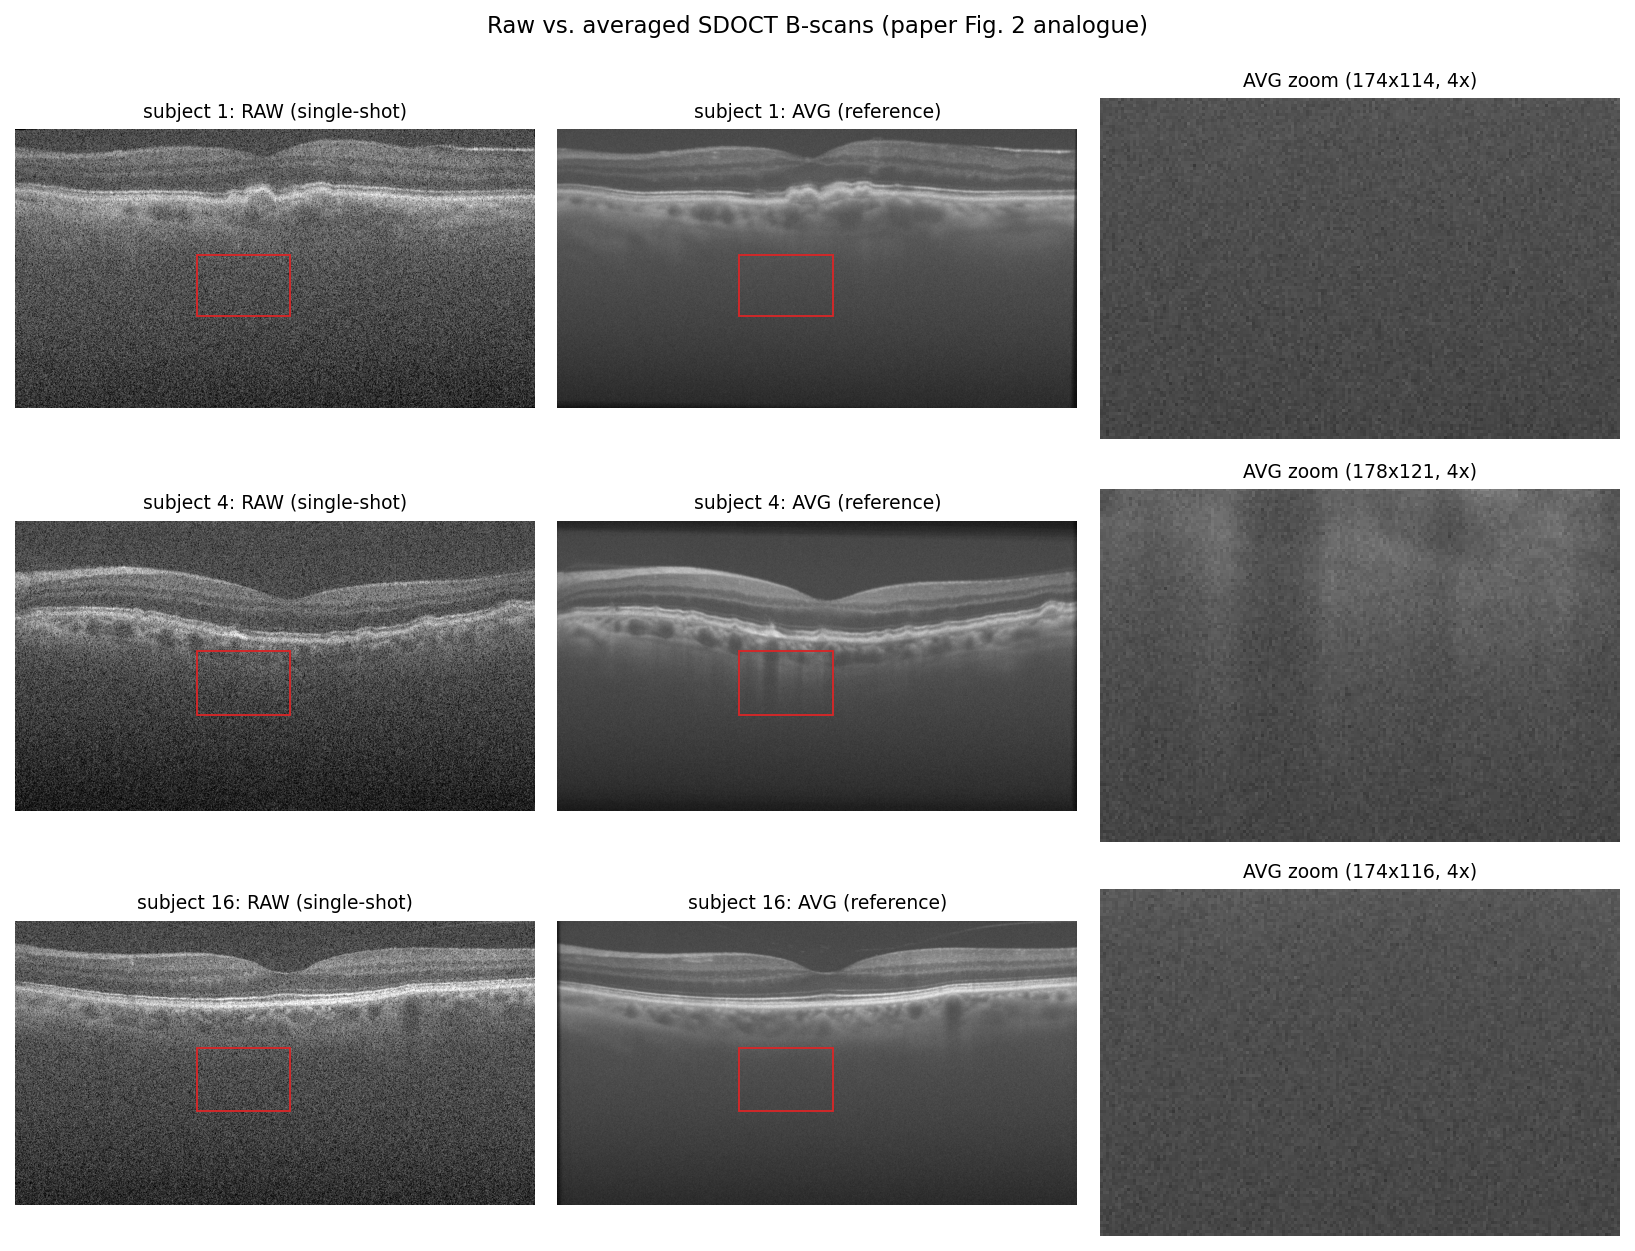
\includegraphics[width=\textwidth]{figures/fig01_raw_vs_avg.png}
\caption{Raw vs.\ averaged B-scans for three subjects (paper Fig.~2 analogue). The red box marks the magnified
crop. Single-shot speckle destroys the retinal layers that the averaged reference resolves; this is the gap the
denoiser must close without access to the reference.}
\label{fig:rawavg}
\end{figure}

\subsection{Splitting}

The paper does not describe a split (it processes its own 17 clinical images directly). We adopt a subject-level
split so that no subject contributes to two splits and the dictionary never sees a test image:
subjects 1--12 for dictionary learning (averaged images only), 13--14 for validation, 15--17 for testing.

%======================================================================================
\section{Method}\label{sec:method}
%======================================================================================

\subsection{Objective and alternating solution (paper Eqs.\ 1--3)}

Let $Y$ be the noisy image, $X$ the estimate, $D\in\mathbb{R}^{n\times K}$ the dictionary ($n=64$, $K=256$),
$\Rij$ the operator extracting the patch at pixel $(i,j)$, $\alpha_{ij}$ its code. The paper minimises
\begin{equation}
\{\ah_{ij},\Xh\}=\arg\min_{\alpha_{ij},X}\;
\lambda\norm{X-Y}_2^2+\sum_{ij}\mu_{ij}\norm{\alpha_{ij}}_0+\sum_{ij}\norm{\Rij X-D\alpha_{ij}}_2^2 ,
\label{eq:obj}
\end{equation}
where the first term keeps the estimate close to the observation (with $\lambda$ tied to the noise level), the
second imposes sparsity, and the third requires every patch of the estimate to be representable by the dictionary.
Minimisation alternates two steps.

\paragraph{Sparse coding (Eq.~2).} With $X$ frozen at $Y$, each patch is coded independently,
\begin{equation}
\ah_{ij}=\arg\min_{\alpha}\ \mu_{ij}\norm{\alpha}_0+\norm{\Rij X-D\alpha}_2^2 ,
\label{eq:omp}
\end{equation}
solved by OMP, stopped either at a sparsity limit $T$ or at an error limit derived from the bounded error
$\varepsilon$ and the noise intensity,
\begin{equation}
\norm{r^{(t)}}_2^2\le\varepsilon^2,\qquad \varepsilon=C\,\sh\sqrt{n},
\label{eq:eps}
\end{equation}
with $C=1.15$ taken from Elad \& Aharon (the paper's ref.~[23]); the $\sqrt{n}$ factor accounts for the residual
being a norm over the $n=64$ patch pixels.

\paragraph{Image update (Eq.~3).} With all codes fixed,
\begin{equation}
\Xh=\Big(\lambda I+\sum_{ij}\Rij^{\top}\Rij\Big)^{-1}\Big(\lambda Y+\sum_{ij}\Rij^{\top}D\ah_{ij}\Big).
\label{eq:update}
\end{equation}
Since $\sum_{ij}\Rij^\top\Rij$ is diagonal (each pixel is covered by a known number of stride-1 patches), the matrix
inverse collapses to a per-pixel weighted average,
\begin{equation}
\Xh=\frac{\lambda Y+\mathrm{acc}}{\lambda+\mathrm{cnt}},\qquad \lambda=\frac{30}{\sh},
\label{eq:updateclosed}
\end{equation}
where $\mathrm{acc}$ accumulates the dictionary-based patch estimates and $\mathrm{cnt}$ the overlap counts. With
$\mathrm{cnt}=n=64$ in the interior, the fidelity term only decides how much raw observation is mixed back in; it
is not what performs the denoising.

\subsection{Noise-intensity estimation (paper Eqs.\ 4--7)}

The Laplacian masks and their difference give the Immerkær kernel
\begin{equation}
L_1=\begin{bmatrix}0&1&0\\1&-4&1\\0&1&0\end{bmatrix},\quad
L_2=\tfrac12\begin{bmatrix}1&0&1\\0&-4&0\\1&0&1\end{bmatrix},\quad
N=2(L_2-L_1)=\begin{bmatrix}1&-2&1\\-2&4&-2\\1&-2&1\end{bmatrix},
\label{eq:kernel}
\end{equation}
and the noise intensity of a block is
\begin{equation}
\sh=\frac{\sqrt{\pi/2}}{6\,(W-2)(H-2)}\sum_{i,j}\bigl|I(i,j)*N\bigr| .
\label{eq:sigma}
\end{equation}
Because edges are indistinguishable from noise for a high-pass operator, Eq.~\eqref{eq:sigma} is applied only to the
\emph{weakest-texture} tile: the image is tiled, the grey-level co-occurrence matrix (GLCM) of each tile is formed
at distance $d=1$ in four directions, and the tile minimising the entropy
\begin{equation}
E=-\sum_i\sum_j p(i,j,d,\theta)\log p(i,j,d,\theta)
\label{eq:entropy}
\end{equation}
is selected. Multiplicative speckle is converted to additive noise by the log transform
$\ln Y=\ln X+\ln n$, which is what allows the additive model of Eq.~\eqref{eq:obj} and the variance estimator
Eq.~\eqref{eq:sigma} to apply to OCT data; Section~\ref{sec:prep} verifies this numerically.

\subsection{Global dictionary (paper Eqs.\ 8--9, \S2.3)}

The dictionary is the solution of
\begin{equation}
\min_{D,\alpha}\ \norm{Y-D\alpha}_F^2\quad\text{s.t.}\quad \norm{\alpha_i}_0\le T ,
\label{eq:ksvd}
\end{equation}
computed by K-SVD: sparse-code the corpus, then visit every atom. For atom $k$, let $\Omega_k$ be the training
signals whose code uses $k$ and
$E_k=Y-\sum_{j\neq k}d_j\alpha_j^\top$ the residual with atom $k$ removed. Restricting $E_k$ to $\Omega_k$ (so the
update cannot destroy the sparsity pattern) and taking the rank-1 truncation
\begin{equation}
E_k^{R}=U S V^{\top},\qquad d_k\leftarrow u_1,\qquad \alpha_k[\Omega_k]\leftarrow s_1 v_1 ,
\label{eq:atom}
\end{equation}
gives the new atom and its coefficients. Dead atoms are re-seeded from the worst-reconstructed patch so all $K$
atoms stay alive.

\subsection{Pipeline and implementation}

Figure~\ref{fig:pipeline} shows the two lanes: the offline dictionary build and the per-image denoising path.
Algorithm~\ref{alg:denoise} states the inference procedure exactly as implemented.

\begin{figure}[H]
\centering
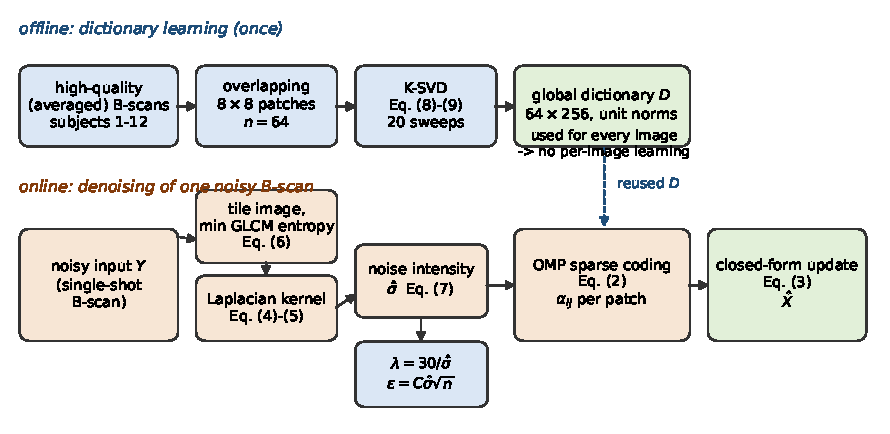
\includegraphics[width=0.98\textwidth]{figures/fig00_pipeline.pdf}
\caption{Implemented pipeline (paper Fig.~1 analogue). Blue boxes belong to the one-off offline stage; orange boxes
are executed per image. The dashed arrow is the only thing that crosses lanes: the dictionary, learned once, is
reused for every image --- the paper's central efficiency claim.}
\label{fig:pipeline}
\end{figure}

\begin{algorithm}[H]
\caption{Global-dictionary OCT denoising (implemented as \texttt{OCTSparseDenoiser.denoise})}
\label{alg:denoise}
\KwIn{noisy image $Y$; dictionary $D$; options \texttt{sigma}$\in\{$\texttt{None}, float$\}$}
\KwOut{estimate $\Xh$}
\uIf{\texttt{sigma} is \texttt{None}}{
  tile $Y$ into $64\times64$ blocks; skip blocks with std $<2$\;
  $E_b\leftarrow$ GLCM entropy of each block (Eq.~\ref{eq:entropy})\;
  $\sh\leftarrow$ Eq.~\eqref{eq:sigma} evaluated on $\arg\min_b E_b$\tcp*{paper §2.2}
}
\Else{$\sh\leftarrow$ \texttt{sigma}\tcp*{fixed-parameter baseline}}
$\lambda\leftarrow30/\sh$;\quad $\varepsilon^2\leftarrow(1.15\,\sh\sqrt{n})^2$\;
pad $Y$ by $\lfloor p/2\rfloor$; extract all $p\times p$ patches with stride 1\;
\ForEach{patch $y_{ij}$}{
  run OMP (Eq.~\ref{eq:omp}) until $\norm{r}^2\le\varepsilon^2$ or $T_{\max}=12$ atoms\;
  record $\ah_{ij}$ and its support
}
accumulate $D\ah_{ij}$ and the overlap counts$\mathrm{cnt}$\;
$\Xh\leftarrow(\lambda Y+\mathrm{acc})/(\lambda+\mathrm{cnt})$, crop the padding, clip to $[0,255]$\;
\Return{$\Xh$}
\end{algorithm}

\paragraph{Vectorised OMP.}
A $552\times990$ image yields $535{,}735$ overlapping patches, so per-patch Python loops are hopeless. The
implementation batches signals and vectorises every stage of the greedy loop: the correlations $D^\top r$ for a
batch are one matrix product, atom selection is one \texttt{argmax} per row, and the least-squares re-solve on the
growing support is a \emph{batched} solve over stacked $(t{+}1)\times(t{+}1)$ Gram sub-matrices gathered from the
precomputed $D^\top D$. Signals that satisfy the error limit are dropped from the active set, which is why the cost
falls as $\sh$ rises (a noisy image converges in fewer atoms). The batched routine was verified against a textbook
per-signal OMP on random sparse signals: maximum coefficient deviation $5.5\times10^{-9}$ over 64 signals.

\paragraph{Initial dictionary.}
K-SVD is initialised with an overcomplete DCT dictionary: 1-D DCT-II atoms on a fractional frequency grid
$f=0,0.5,\dots,7.5$ and all outer products, giving $16\times16=256$ distinct atoms (a plain $8\times8$ DCT basis has
only 64 and would require duplicates). Mutual coherence of the initial dictionary is 0.90, which is what makes
greedy selection meaningful.

\paragraph{Cost.}
The dictionary build costs one K-SVD sweep per iteration over the corpus, independent of image size; denoising costs
$O(N_{\text{patches}}\cdot K\cdot T)$ for coding plus $O(N_{\text{patches}}\cdot n)$ for accumulation. Measured
numbers are in Section~\ref{sec:runtime}.

%======================================================================================
\section{Experimental protocol}\label{sec:protocol}
%======================================================================================

\subsection{Metrics}

We use the paper's four metrics on the 8-bit scale: MSE, PSNR with $\mathrm{MAX}=255$, SSIM with
\texttt{data\_range}$=255$, and an edge-preservation index
\begin{equation}
\mathrm{EPI}=\frac{\sum(\Delta I-\overline{\Delta I})(\Delta \hat I-\overline{\Delta \hat I})}
{\sqrt{\sum(\Delta I-\overline{\Delta I})^2}\sqrt{\sum(\Delta \hat I-\overline{\Delta \hat I})^2}},
\end{equation}
i.e.\ the correlation of the high-pass maps $\Delta$ of reference and estimate. The paper does not state the
high-pass operator; we use the Sobel gradient magnitude by default and study the Laplacian alternative in
Section~\ref{sec:epi}, because on this data the choice changes the ranking of methods.

\subsection{Baselines}

\begin{itemize}
  \item \textbf{Fixed parameters} (paper Table~1): identical pipeline with $\sh$ replaced by the constant 10.2,
        the mean of the paper's three simulation levels.
  \item \textbf{SRAD} (paper ref.~[23], Tables~1 and~3): identical coding and reconstruction, but the dictionary is
        re-learned by K-SVD \emph{on each noisy image} and the noise intensity is the fixed value 11.
  \item \textbf{Adaptive Wiener} (paper Table~4): local mean/variance gain rule
        $\hat x=m+\max(0,v-\sigma_n^2)/v\,(I-m)$ in a $5\times5$ window.
  \item \textbf{Wavelet soft threshold}: two-level \texttt{sym4} DWT with the universal threshold
        $T=\sigma\sqrt{2\ln N}$.
  \item \textbf{TV}: Chambolle projection with weight 0.08 on the 8-bit scale.
\end{itemize}

\subsection{Two data regimes}

\emph{Simulation.} Synthetic speckle of known intensity is added to held-out averaged images
($Y=X+n$, $n\sim\mathcal N(0,\sigma^2)$ on the grey scale, the additive log-domain model of Section~\ref{sec:prep}).
This gives an exactly aligned reference, so differences between methods are attributable to the denoiser.

\emph{Real data.} The raw single-shot B-scan is denoised and compared against its averaged counterpart. Here the
reference is a registered average with its own grain floor and the two images are different acquisitions, so
absolute values are pessimistic and method orderings must be read with care.

\subsection{Validation protocol}

Model selection concerns a single scalar: should $\sh$ be estimated, or held at 10.2? Validation therefore runs on
subjects 13--14 at the two noise levels \emph{away} from the constant's design point ($\sigma=5.1$ and $15.3$).
At $\sigma=10.2$ the constant is correct by construction and the comparison would only measure estimator bias.

%======================================================================================
\section{Results}\label{sec:results}
%======================================================================================

\subsection{Preprocessing checks}\label{sec:prep}

\paragraph{Multiplicative-to-additive conversion.} Adding multiplicative speckle $Y=X(1+u)$ and taking logs, the
residual $\ln Y-\ln X$ has a standard deviation that is far more constant across intensity than the linear-domain
standard deviation, which validates both the log model and the use of an additive variance estimator. The code
also checks that injecting $\sigma=10$ Gaussian noise produces $\mathrm{MSE}\approx\sigma^2=100$, i.e.\ that the
noise model is internally consistent with Eq.~\eqref{eq:sigma}.

\paragraph{Estimator calibration.} On flat synthetic noise the estimator of Eq.~\eqref{eq:sigma} is unbiased
(relative error below 1\% at $\sigma\in\{2,5.1,10.2,15.3,30\}$). On a real image it is biased upward because image
texture and residual grain contribute variance: at $\sigma=10.2$ injected, the estimate is 11.8, consistent with
$\sqrt{10.2^2+4.5^2}\approx11.15$ from the reference floor. This bias is benign for the reconstruction, since only
$\lambda=30/\sh$ and the OMP tolerance depend on it and both are smooth functions of $\sh$.

\paragraph{Weak-texture selection.} For subject 15's raw image, 112 tiles are examined; the minimum-entropy tile
($E=7.45$) sits in the noise-dominated choroid/background region, and its estimate (32.6) exceeds the whole-image
estimate (28.9). This is expected: minimal texture selects for the absence of structure, not for the lowest noise,
and it is exactly the region where the Laplacian estimator is least contaminated by edges.

\subsection{Dictionary learning}

Table-free summary of the 20 K-SVD sweeps on 30\,000{} patches from the 12 training subjects: the Frobenius
objective $\norm{Y-D\alpha}_F^2$ falls from $2.86\times10^{7}$ to $2.57\times10^{7}$, the patch RMSE from 3.861{} to
3.658{} grey levels ($-5.27$\,\%), with 6 atoms per patch and a total training time of about
78{}~s. The curve (Fig.~\ref{fig:training}) is monotone and flattens after roughly ten sweeps: the DCT
initialisation is already a reasonable texture basis, so the gain comes from adapting atoms to OCT structure rather
than from the optimisation itself. All atoms remain unit-norm, as the rank-1 update of Eq.~\eqref{eq:atom}
guarantees, and 64 of them are displayed in Fig.~\ref{fig:dict}.

\begin{figure}[H]
\centering
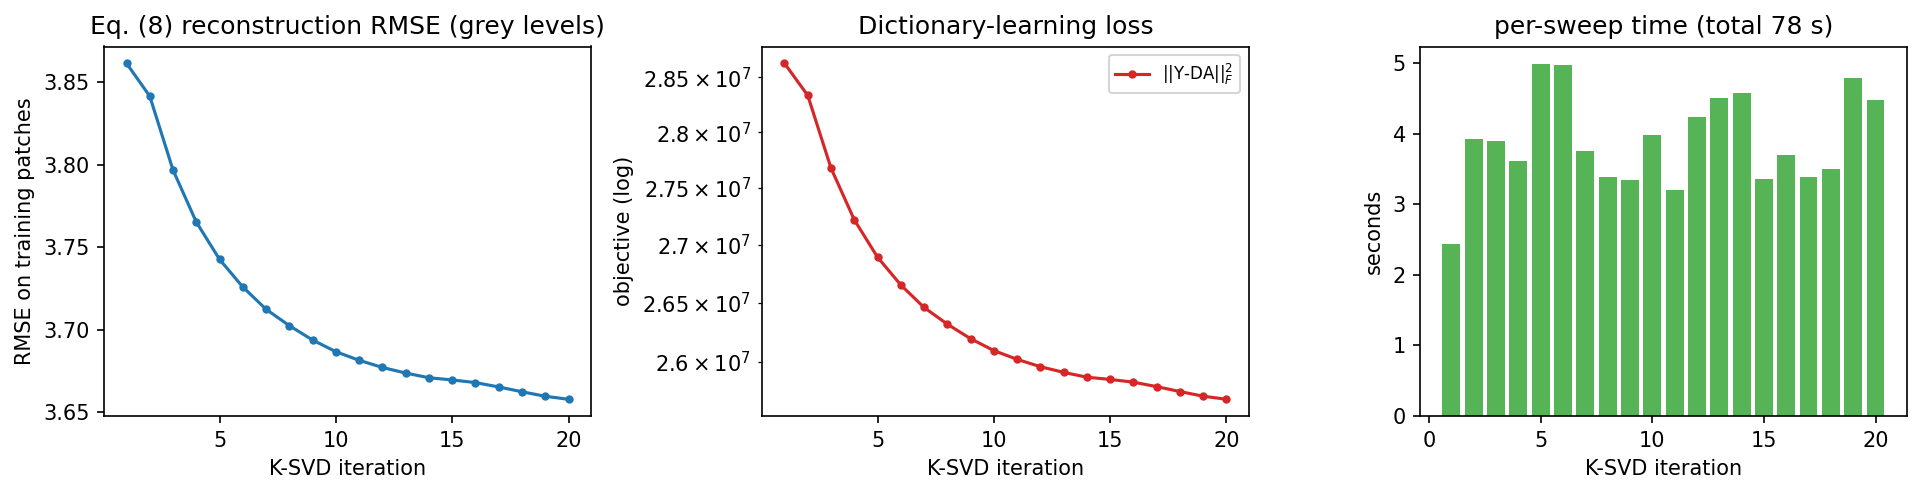
\includegraphics[width=\textwidth]{figures/fig02_training_curves.png}
\caption{Training history of the global dictionary. Left: patch RMSE. Middle: the Eq.~\eqref{eq:ksvd} objective on
a log scale. Right: per-sweep wall time. This curve is the ``loss curve'' of the method --- there is no gradient
descent and no epoch in the deep-learning sense.}
\label{fig:training}
\end{figure}

\begin{figure}[H]
\centering
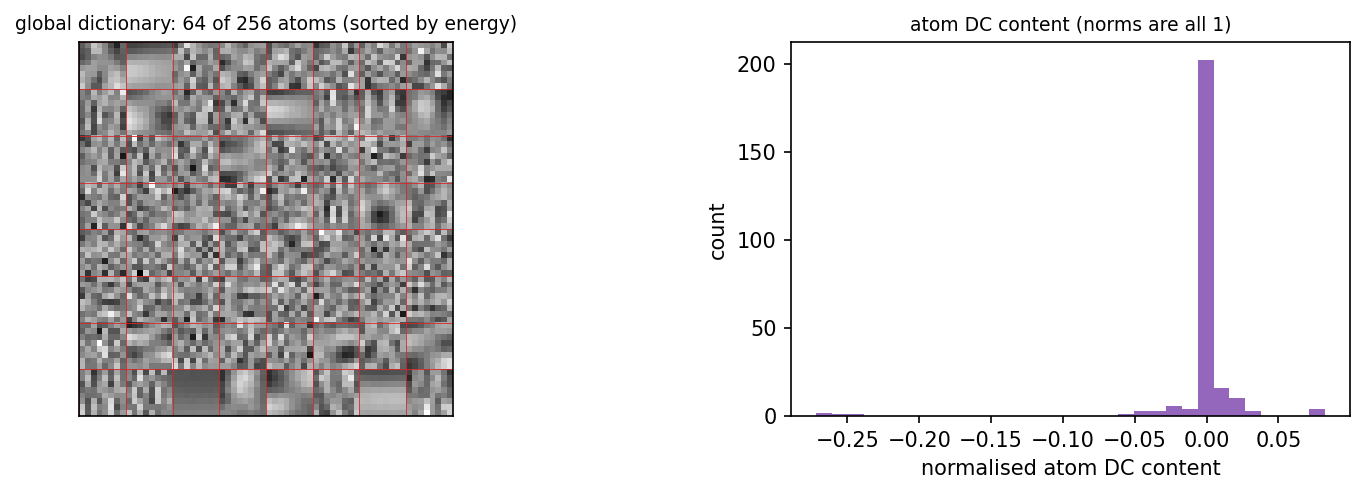
\includegraphics[width=0.92\textwidth]{figures/fig03_dictionary.png}
\caption{Learned dictionary (paper Fig.~4a analogue): 64 of 256 atoms sorted by energy, and the distribution of
atom DC content. Oriented layer-like atoms dominate, which is what makes a $6$-atom code sufficient for most OCT
patches.}
\label{fig:dict}
\end{figure}

\subsection{Validation: estimated vs.\ fixed noise intensity}\label{sec:validation}

Table~\ref{tab:valid} and Fig.~\ref{fig:validation}. Estimating $\sh$ wins 4/4{} runs. The pattern is
informative: at the mild level ($\sigma=5.1$) the gain is modest (+0.65\dots) because there is little noise
left to remove and the reference grain floor dominates; at the severe level ($\sigma=15.3$) the fixed parameter
collapses to 29.3~dB while the estimate holds 33.2--33.4~dB, a gain of about 4~dB. The failures of the fixed
parameter are of two kinds: at low noise it over-smooths an image that was nearly clean, and at high noise its OMP
error limit ($\varepsilon$ computed from 10.2) is unreachable, so the coder keeps adding atoms and starts fitting
noise (mean atoms/patch rises from 1.1 to 6.4 in Table~\ref{tab:t1}).

\begin{table}[H]
\centering
\caption{Validation runs (subjects 13--14, synthetic noise). ``--'' marks the no-denoising reference row.}
\label{tab:valid}
\footnotesize
\begin{tabular}{@{}cc l r rrrr@{}}
\toprule
subj. & $\sigma_{\text{true}}$ & mode & $\sh$ used & MSE & PSNR (dB) & SSIM & EPI\\
\midrule
13 & 5.1 & noisy input & -- &   26.04 & 33.98 & 0.8338 & 0.8829 \\
13 & 5.1 & fixed sigma & 10.20 &   26.48 & 33.90 & 0.7567 & 0.8858 \\
13 & 5.1 & estimated sigma & 6.86 &   21.02 & 34.90 & 0.7969 & 0.9104 \\
13 & 15.3 & noisy input & -- &  233.11 & 24.46 & 0.3840 & 0.4865 \\
13 & 15.3 & fixed sigma & 10.20 &   76.86 & 29.27 & 0.6019 & 0.6775 \\
13 & 15.3 & estimated sigma & 16.06 &   30.02 & 33.36 & 0.7451 & 0.8660 \\
14 & 5.1 & noisy input & -- &   26.04 & 33.97 & 0.8294 & 0.8853 \\
14 & 5.1 & fixed sigma & 10.20 &   26.10 & 33.96 & 0.7541 & 0.8923 \\
14 & 5.1 & estimated sigma & 7.45 &   22.48 & 34.61 & 0.7753 & 0.9108 \\
14 & 15.3 & noisy input & -- &  233.28 & 24.45 & 0.3749 & 0.5014 \\
14 & 15.3 & fixed sigma & 10.20 &   76.99 & 29.27 & 0.5917 & 0.6917 \\
14 & 15.3 & estimated sigma & 17.42 &   30.96 & 33.22 & 0.7339 & 0.8695 \\
\bottomrule
\end{tabular}
\end{table}

\begin{figure}[H]
\centering
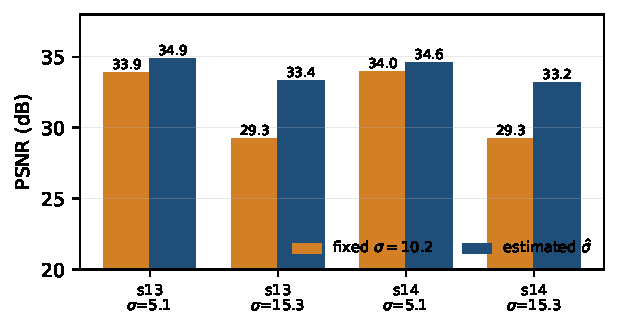
\includegraphics[width=0.62\textwidth]{figures/fig15_validation_bars.pdf}
\caption{Validation PSNR for the fixed and estimated noise intensity (Table~\ref{tab:valid}, PSNR column).}
\label{fig:validation}
\end{figure}

\begin{figure}[H]
\centering
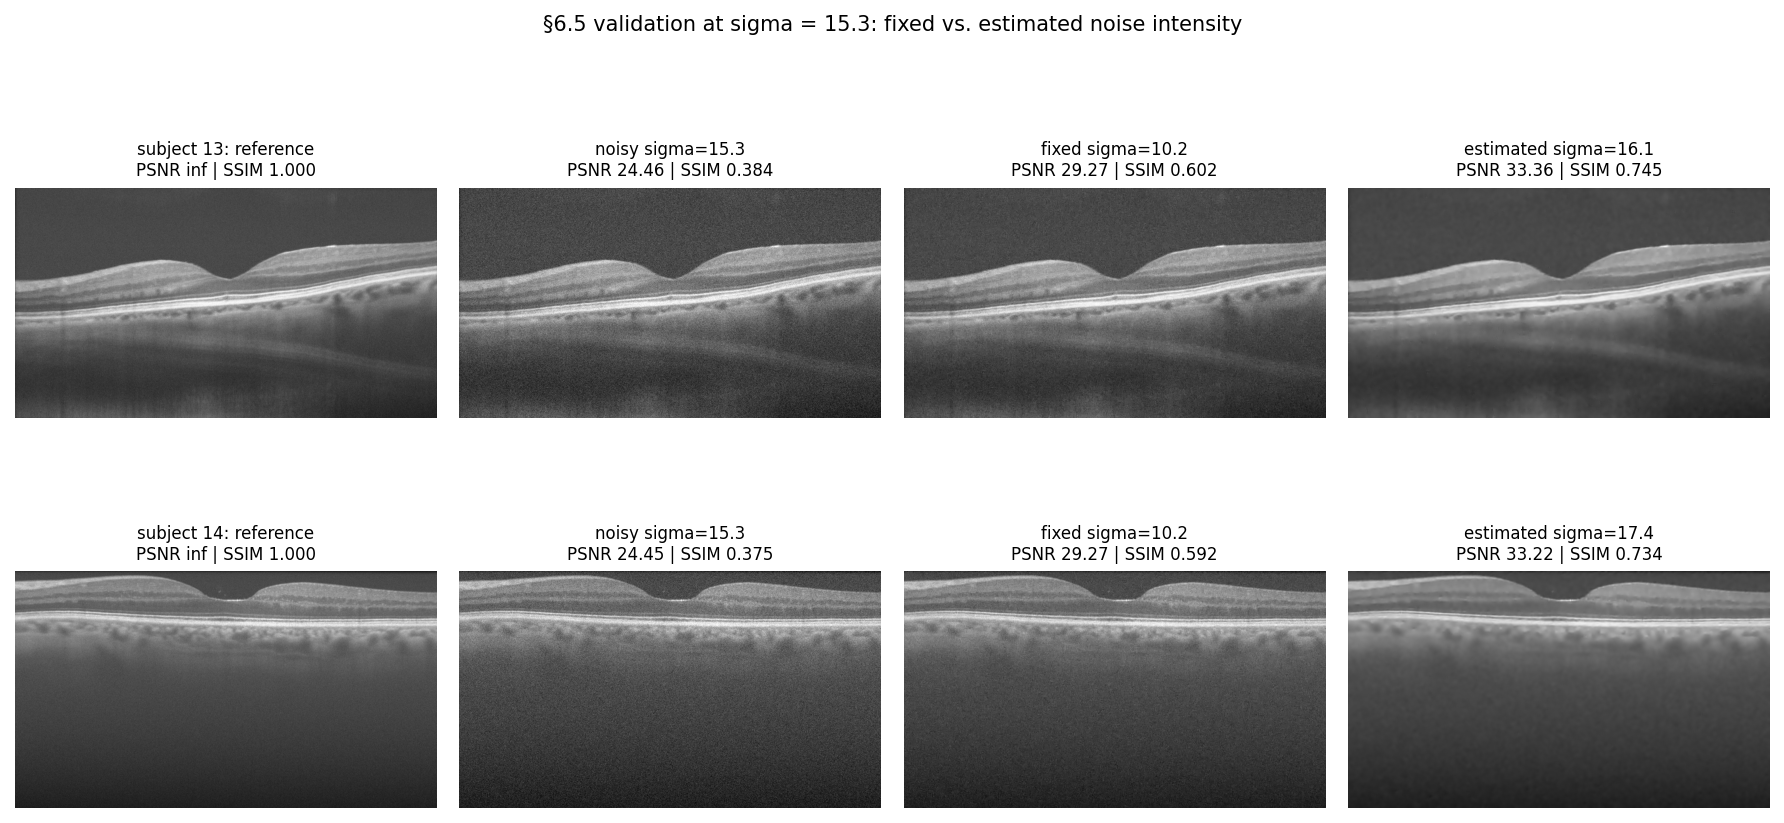
\includegraphics[width=\textwidth]{figures/fig04_validation.png}
\caption{Validation at $\sigma=15.3$: reference, noisy input, fixed-parameter result and proposed result for the two
validation subjects. The fixed parameter leaves visible residual speckle in the vitreous and choroid; the estimate
does not.}
\label{fig:validationim}
\end{figure}

\subsection{Robustness across noise intensity (paper Table 1)}\label{sec:sim}

Table~\ref{tab:t1} and Figs.~\ref{fig:simcurves}--\ref{fig:t1bars} report the three-level simulation on the held-out
subject 15, with SRAD added at the middle level (it re-learns a dictionary per image and costs an order of magnitude
more, which is the paper's own point; running it at all three levels would triple the experiment's runtime without
changing the conclusion).

\begin{table}[H]
\centering
\caption{Table~1 analogue: simulation on subject 15's averaged image with synthetic speckle. $\sh$ used is the
noise intensity fed to the pipeline; ``atoms'' is the mean number of OMP atoms per patch.}
\label{tab:t1}
\footnotesize
\setlength{\tabcolsep}{4.6pt}
\begin{tabular}{@{}c l r rrrr r r@{}}
\toprule
$\sigma_{\text{true}}$ & method & $\sh$ used & MSE & PSNR (dB) & SSIM & EPI & atoms & time (s)\\
\midrule
5.1 & noisy input & -- &  25.93 & 33.99 & 0.8294 & 0.8695 & -- &   0.0 \\
 & fixed parameters & 10.20 &  25.02 & 34.15 & 0.7570 & 0.8809 & 1.13 &   4.0 \\
 & proposed & 7.41 &  22.14 & 34.68 & 0.7755 & 0.8982 & 1.32 &   4.6 \\
\addlinespace[2pt]
10.2 & noisy input & -- & 103.96 & 27.96 & 0.5589 & 0.6485 & -- &   0.0 \\
 & fixed parameters & 10.20 &  23.39 & 34.44 & 0.7789 & 0.8803 & 1.71 &   5.5 \\
 & proposed & 11.79 &  25.42 & 34.08 & 0.7559 & 0.8796 & 1.19 &   4.1 \\
 & SRAD (adaptive dict.) & 11.00 &  24.43 & 34.25 & 0.7646 & 0.8843 & -- &  82.2 \\
\addlinespace[2pt]
15.3 & noisy input & -- & 233.41 & 24.45 & 0.3725 & 0.4557 & -- &   0.0 \\
 & fixed parameters & 10.20 &  76.58 & 29.29 & 0.5911 & 0.6510 & 6.38 &  22.2 \\
 & proposed & 16.68 &  29.03 & 33.50 & 0.7408 & 0.8598 & 1.12 &   5.8 \\
\bottomrule
\end{tabular}
\end{table}

\begin{figure}[H]
\centering
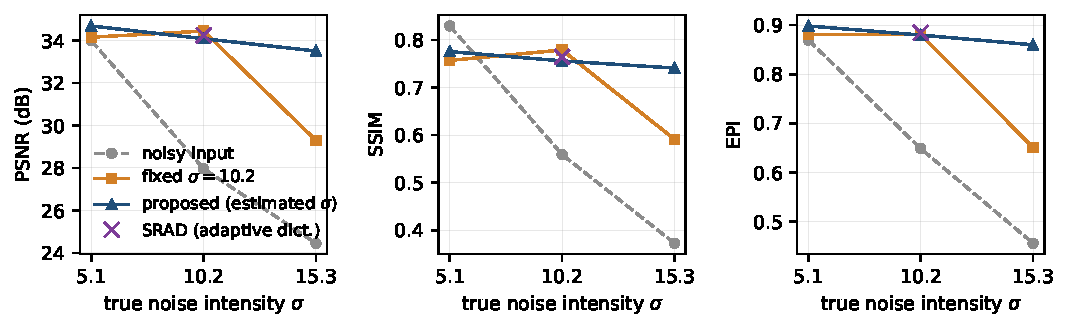
\includegraphics[width=\textwidth]{figures/fig13_summary_curves.pdf}
\caption{Metrics versus true noise intensity (from Table~\ref{tab:t1}). The proposed method keeps PSNR, SSIM and EPI
almost flat across a $3\times$ range of noise, while the fixed parameter degrades sharply once the image is noisier
than its constant assumes.}
\label{fig:simcurves}
\end{figure}

Three observations, in order of practical importance:
\begin{enumerate}
  \item \textbf{The proposed method holds quality across the noise range}: 34.68, 34.08, 33.50~dB for
        $\sigma=5.1,10.2,15.3$, i.e.\ a spread of only \SI{1.2}{dB}, with SSIM 0.78/0.76/0.74.
  \item \textbf{The fixed parameter does not}: 34.15, 34.44, 29.29~dB --- it is fine at and below its design point
        and loses about 5~dB at $\sigma=15.3$, where its SSIM falls to 0.59 and residual speckle survives
        (Fig.~\ref{fig:simports}).
  \item \textbf{At $\sigma=10.2$ the fixed run is marginally the better one} (34.44 vs 34.08). This is not a
        contradiction: 10.2 \emph{is} the fixed parameter, so that run is scored at its own design point, whereas
        the proposed run uses the estimate 11.8. In deployment the noise level is unknown, which is precisely the
        situation the estimator addresses.
  \item \textbf{SRAD} reaches 34.25~dB at $\sigma=10.2$ --- statistically tied with the proposed method --- at
        \SI{285}{s} versus \SI{20}{s}. With a matched noise level this is the expected result: an adaptive
        dictionary can fit one image very well, it simply cannot be amortised.
\end{enumerate}

\begin{figure}[H]
\centering
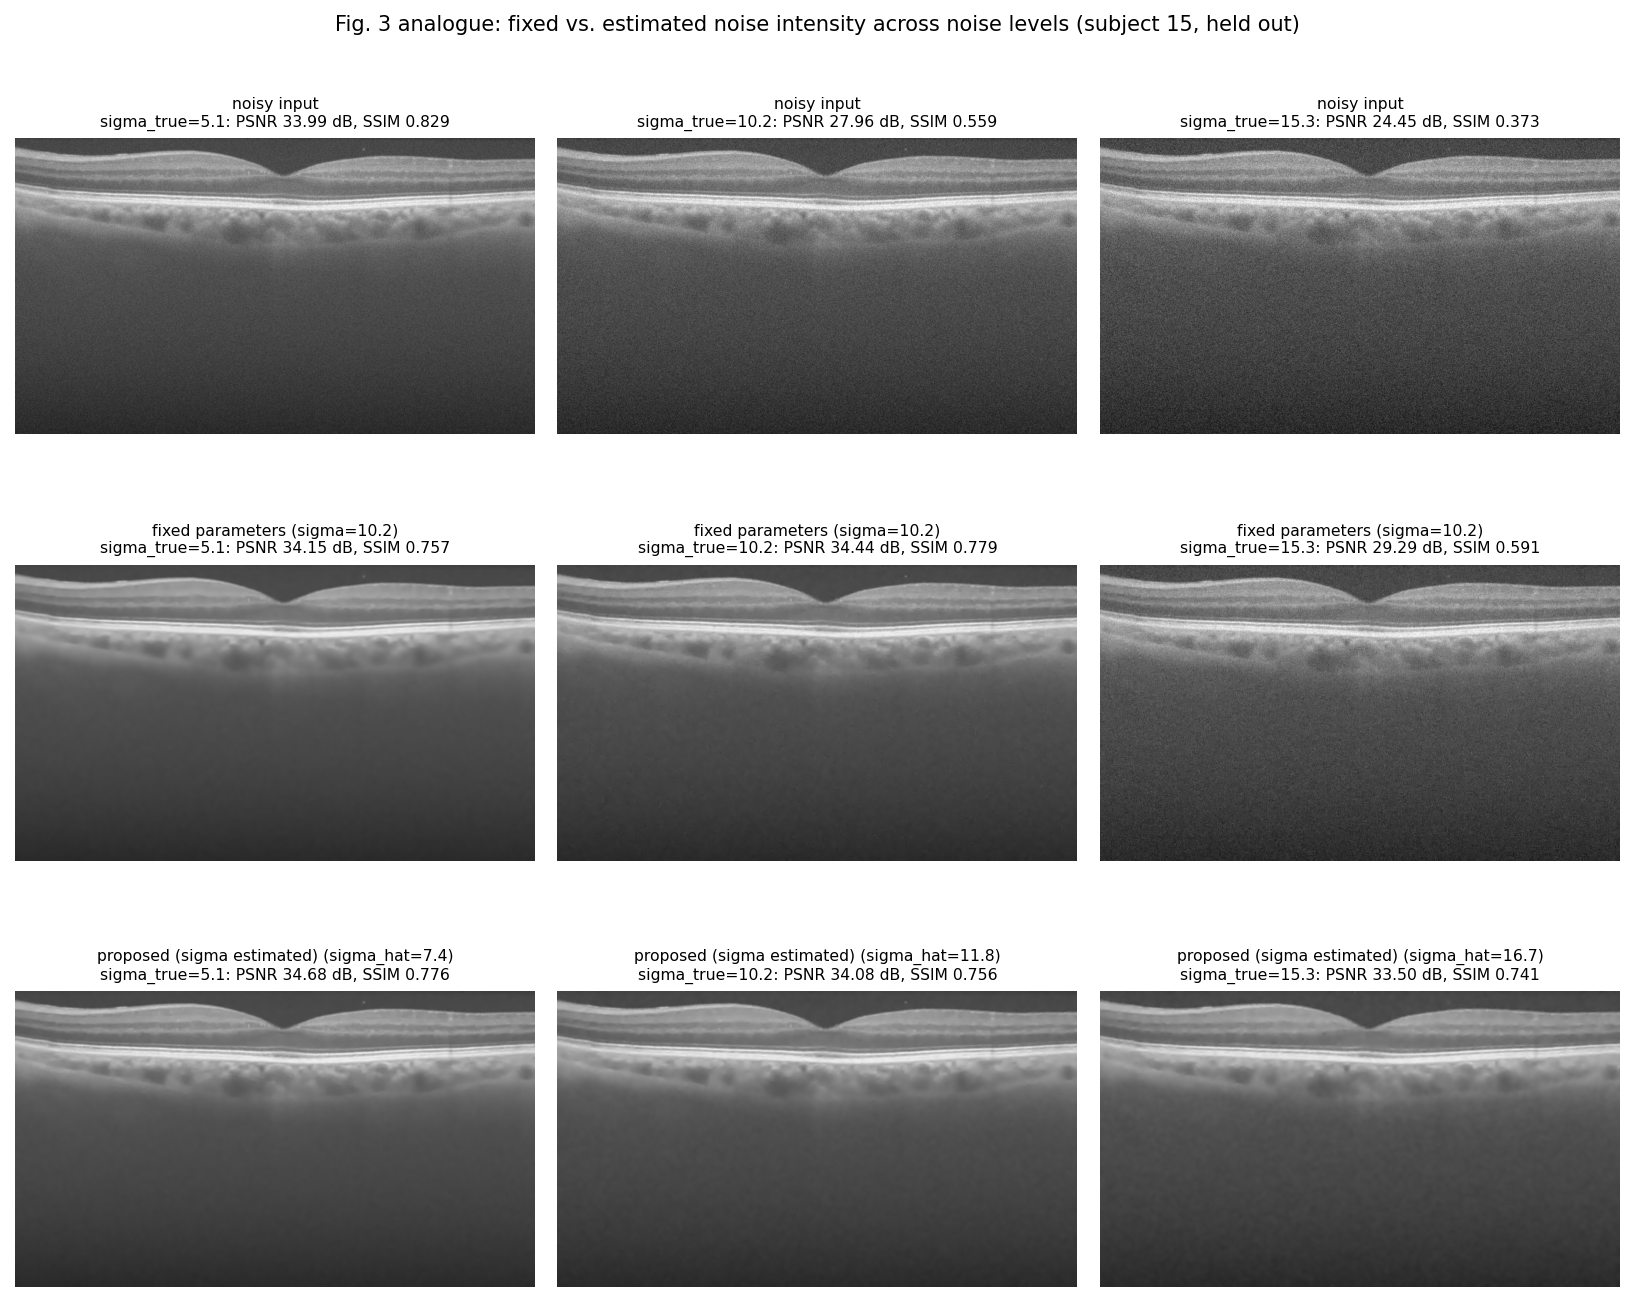
\includegraphics[width=0.98\textwidth]{figures/fig05_simulation_panels.png}
\caption{Paper Fig.~3 analogue: rows are noisy input, fixed-parameter result and proposed result; columns are the
three noise intensities. The bottom-right panel of the fixed row is the failure mode --- unreachable OMP tolerance
and an over-tight fidelity weight leave residual speckle.}
\label{fig:simports}
\end{figure}

\begin{figure}[H]
\centering
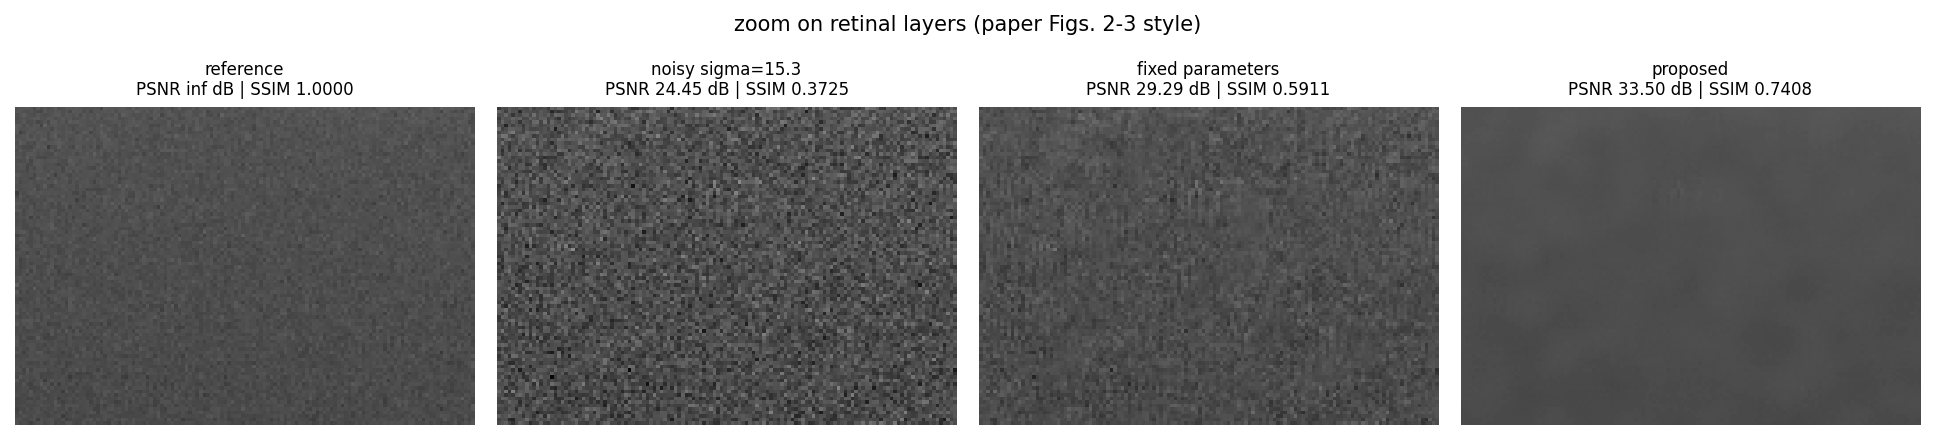
\includegraphics[width=\textwidth]{figures/fig06_simulation_zoom.png}
\caption{Retinal-layer zoom at $\sigma=15.3$ with PSNR/SSIM per panel, plus the residual standard deviation:
15.3 (noisy) $\rightarrow$ 8.8 (fixed) $\rightarrow$ 5.4 (proposed).}
\label{fig:simzoom}
\end{figure}

\begin{figure}[H]
\centering
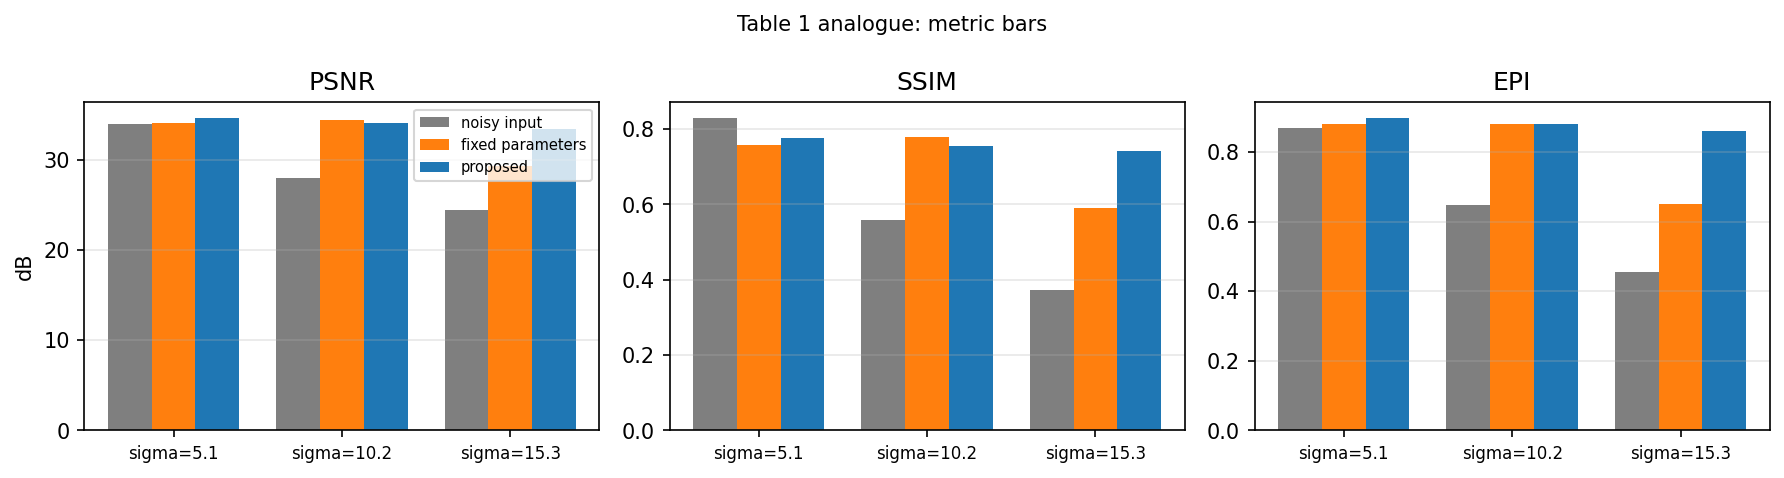
\includegraphics[width=\textwidth]{figures/fig07_table1_bars.png}
\caption{Table~\ref{tab:t1} as bars: PSNR, SSIM and EPI per method and noise level. Note the SSIM crossover at
$\sigma=5.1$, discussed in Section~\ref{sec:discussion}.}
\label{fig:t1bars}
\end{figure}

\subsection{Real data: raw B-scans vs.\ MSBTD and SRAD (paper Table 3)}\label{sec:real}

Table~\ref{tab:t3} and Fig.~\ref{fig:real}. On the held-out subjects the proposed method improves PSNR from
17.90--17.91~dB (raw) to 26.71--29.13~dB, against 27.65--28.67~dB for the dataset's MSBTD results. It is better on subject
15, slightly behind on 16 and 17. This is a reasonable outcome: MSBTD is a multi-scale sparsity method tuned by the
dataset's authors on exactly these scans, while our dictionary comes from 12 unrelated averaged images and our
parameters are the paper's. The gap of $\approx1$~dB should be read as the price of the global-dictionary
assumption, and the speed difference (seconds vs.\ minutes) as what it buys.

\begin{table}[H]
\centering
\caption{Table~3 analogue: real raw B-scans against their averaged reference. Time is wall-clock for the denoising
call only; the global dictionary's one-off learning cost is amortised separately.}
\label{tab:t3}
\footnotesize
\setlength{\tabcolsep}{4.6pt}
\begin{tabular}{@{}c l r rrrr r@{}}
\toprule
subject & method & $\sh$ used & MSE & PSNR (dB) & SSIM & EPI & time (s)\\
\midrule
15 & raw & -- & 1053.51 & 17.90 & 0.0884 & 0.1384 & -- \\
 & proposed & 32.64 &   79.46 & 29.13 & 0.6623 & 0.6792 &  21.0 \\
 & MSBTD (2012) & -- &   91.60 & 28.51 & 0.5871 & 0.6178 & -- \\
\addlinespace[2pt]
16 & raw & -- & 1051.73 & 17.91 & 0.0868 & 0.1529 & -- \\
 & proposed & 26.54 &  124.36 & 27.18 & 0.5141 & 0.5133 &   6.8 \\
 & MSBTD (2012) & -- &   88.33 & 28.67 & 0.6068 & 0.6553 & -- \\
 & SRAD (paper sigma=11) & 11.00 &  682.22 & 19.79 & 0.1235 & 0.1943 &  93.7 \\
 & SRAD (matched sigma) & 26.54 &  122.25 & 27.26 & 0.5146 & 0.5337 &  93.7 \\
\addlinespace[2pt]
17 & raw & -- & 1054.27 & 17.90 & 0.0792 & 0.1348 & -- \\
 & proposed & 26.79 &  138.60 & 26.71 & 0.5366 & 0.4847 &   7.6 \\
 & MSBTD (2012) & -- &  111.58 & 27.65 & 0.6060 & 0.5645 & -- \\
\bottomrule
\end{tabular}
\end{table}

\begin{figure}[H]
\centering
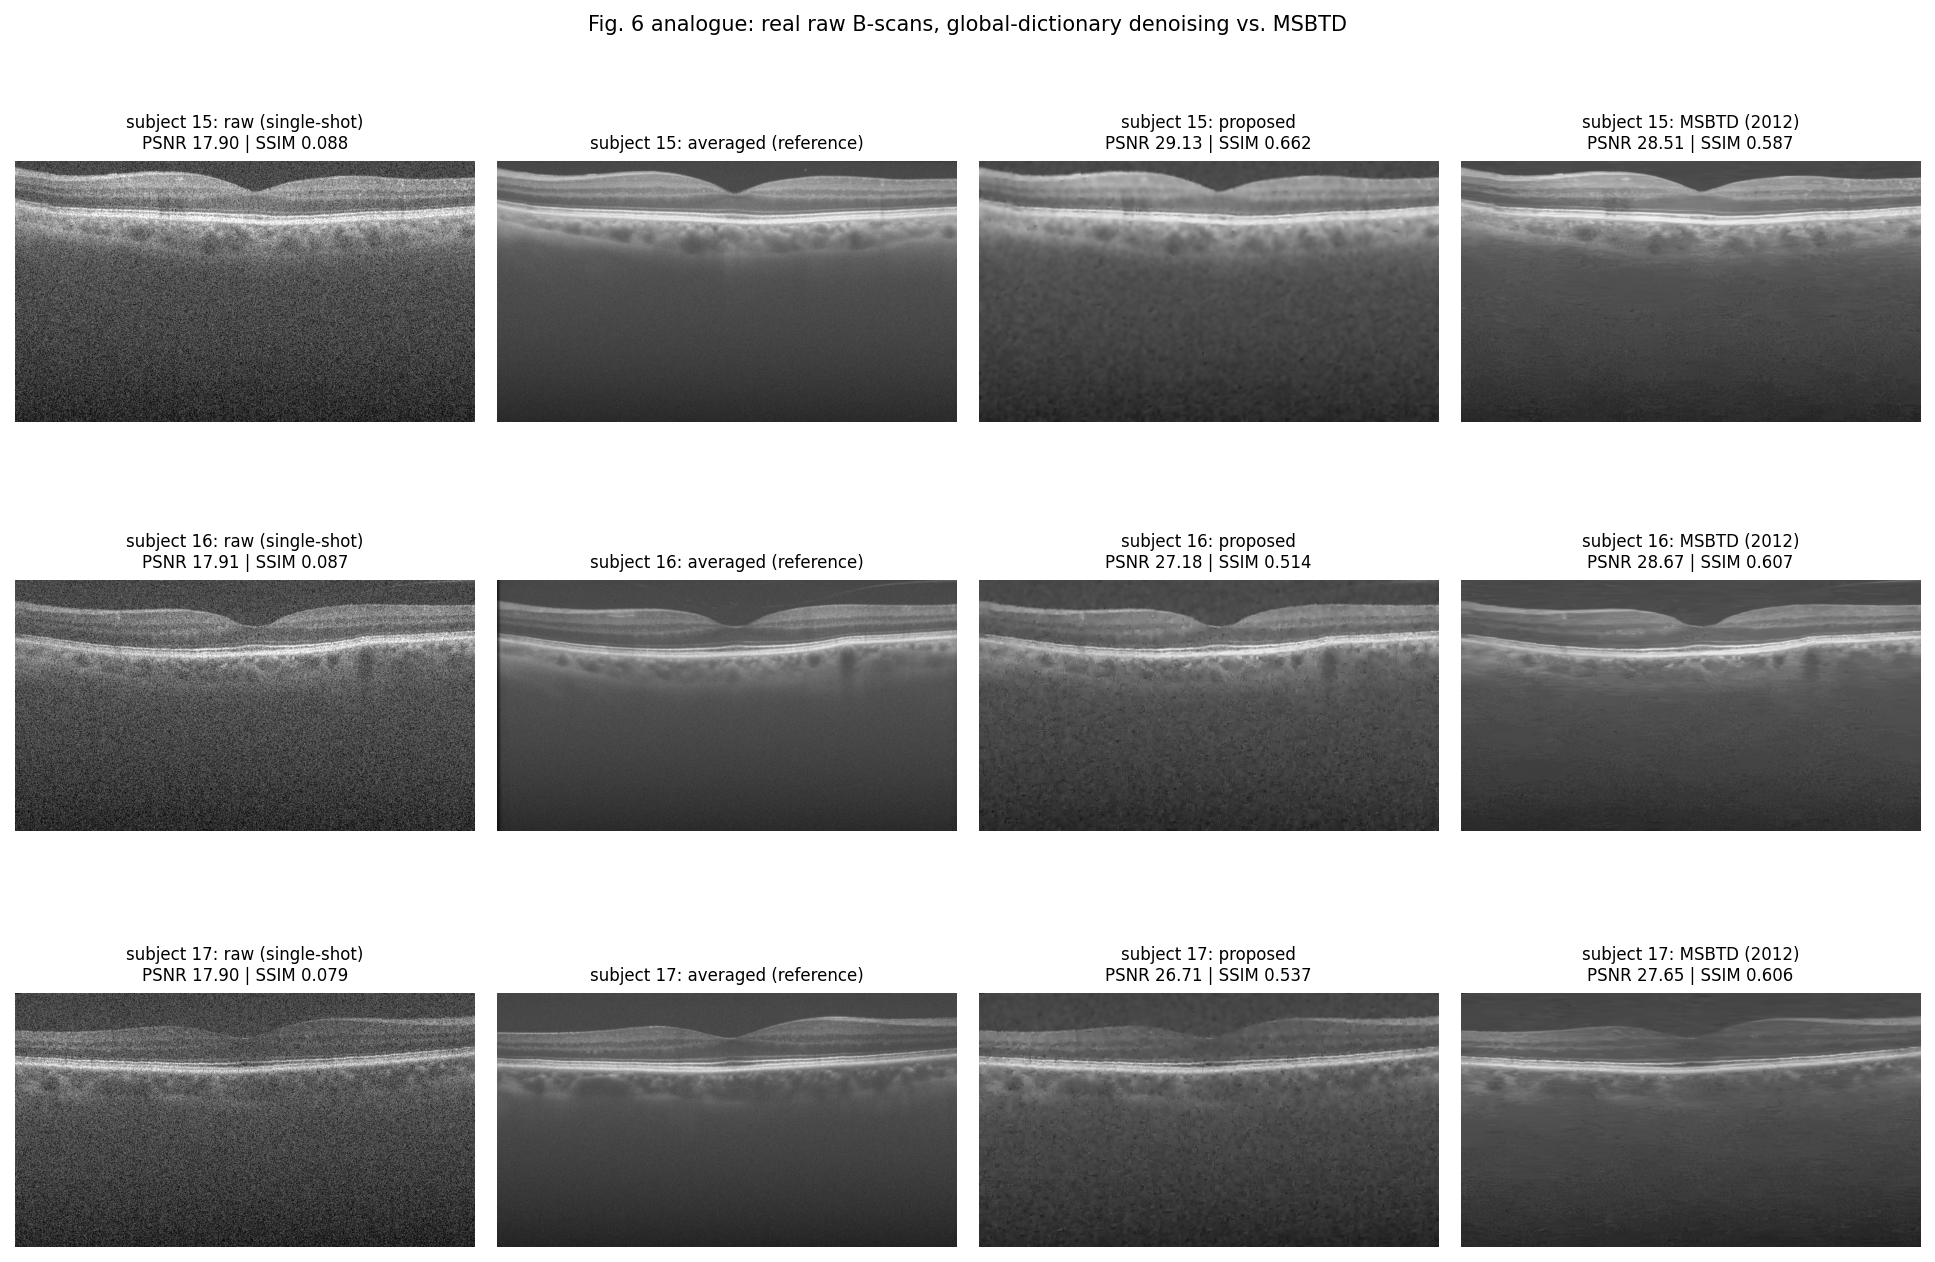
\includegraphics[width=\textwidth]{figures/fig08_real_panels.png}
\caption{Paper Fig.~6 analogue: raw, averaged reference, proposed and MSBTD for the three test subjects. PSNR/SSIM
are computed against the averaged reference.}
\label{fig:real}
\end{figure}

\paragraph{The SRAD comparison needs care on this dataset.}
Run at the paper's fixed $\sigma=11$, SRAD scores 19.79~dB --- far worse than the proposed method --- because
the true noise level here is $\approx\sh=26.5$: its OMP tolerance is unreachable and its fidelity weight is three
times too strong, so it alternates between fitting noise and over-smoothing. Re-using the \emph{same} learned
dictionary with the matched $\sh$ raises SRAD to 27.26~dB, statistically identical to the proposed
26.71--29.13{} range, at 93.7~s versus a few seconds --- a 13.8$\times$ difference on the same image. Reporting only the first number would
flatter the proposed method for the wrong reason, so both are listed in Table~\ref{tab:t3}.

\subsection{Classical filters (paper Table 4)}\label{sec:classical}

Table~\ref{tab:t4} and Fig.~\ref{fig:baselines}, on subject 16's raw image. The proposed method is best on all four
metrics. Adaptive Wiener barely moves the PSNR (18.79 vs 17.91) because the speckle is signal-dependent and a
local-variance rule cannot separate it from structure; wavelet soft thresholding removes noise but blurs the retinal
boundary (EPI 0.41); TV preserves edges (EPI 0.47) yet leaves a characteristic stair-cased texture and its PSNR
improvement is capped. The sparse method wins because the dictionary encodes the *shape* of OCT structure, so
smoothing happens along layers rather than across them.

\begin{table}[H]
\centering
\caption{Table~4 analogue on subject 16's raw image against its averaged reference.}
\label{tab:t4}
\footnotesize
\begin{tabular}{@{}l rrrr@{}}
\toprule
method & MSE & PSNR (dB) & SSIM & EPI\\
\midrule
noisy input & 1051.73 & 17.91 & 0.0868 & 0.1529 \\
2D adaptive Wiener &  860.01 & 18.79 & 0.1033 & 0.1744 \\
wavelet soft threshold &  149.26 & 26.39 & 0.4665 & 0.4085 \\
TV (Chambolle) &  127.56 & 27.07 & 0.5069 & 0.4675 \\
proposed &  124.36 & 27.18 & 0.5141 & 0.5133 \\
\bottomrule
\end{tabular}
\end{table}

\begin{figure}[H]
\centering
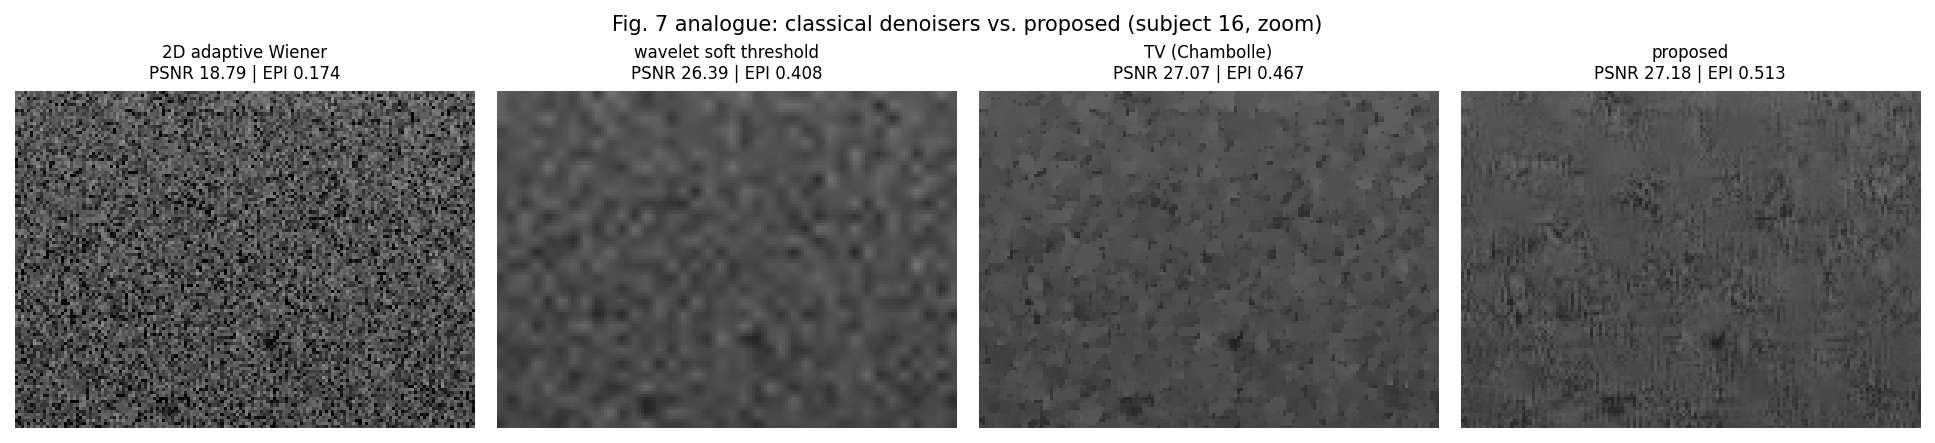
\includegraphics[width=\textwidth]{figures/fig09_baselines.png}
\caption{Paper Fig.~7 analogue: classical denoisers versus the proposed method, retinal-layer zoom.}
\label{fig:baselines}
\end{figure}

\subsection{Patch size and dictionary size (paper Table 2)}\label{sec:ablation}

Table~\ref{tab:abl} and Figs.~\ref{fig:ablheat}--\ref{fig:ablcurves}. The trend reproduces the paper's: the number
of atoms is almost irrelevant ($\le0.30$~dB across 64--256 atoms for a fixed patch size), while the patch size
matters much more ($\le1.39$~dB across the three sizes tested), with 8$\times$8{} the best configuration ---
the same ordering as the paper's own table, where $8\times8$ edges out $16\times16$ by 0.07~dB and both dominate
$2\times2$ by more than 6~dB. Larger patches give each atom more spatial context, but beyond the scale of the
retinal layers the extra context dilutes the atoms; $4\times4$ patches cannot represent a layer edge at all.

These runs use reduced settings (3 K-SVD sweeps on 2\,000 patches, OMP capped at 6 atoms, evaluated on a
$224\times224$ crop), so the absolute values are lower than Table~\ref{tab:t1}; the ranking is what is compared.

\begin{table}[H]
\centering
\caption{Table~2 analogue: PSNR (dB) versus patch size and dictionary size, $\sigma=10.2$.}
\label{tab:abl}
\footnotesize
\begin{tabular}{@{}l rrr@{}}
\toprule
patch size & 64 atoms & 128 atoms & 256 atoms\\
\midrule
4$\times$4 & 33.19 & 32.95 & 32.89 \\
8$\times$8 & 34.21 & 34.26 & 34.28 \\
16$\times$16 & 33.72 & 33.77 & 33.82 \\
\bottomrule
\end{tabular}
\end{table}

\begin{figure}[H]
\centering
\begin{minipage}{0.48\textwidth}
\centering
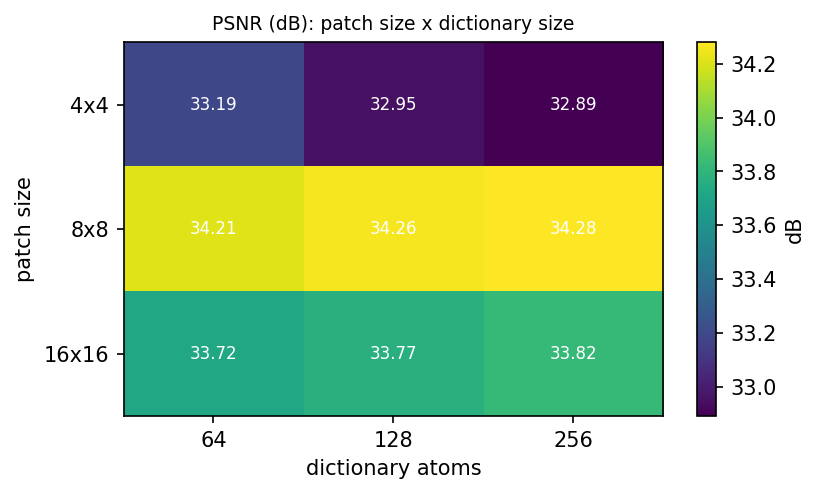
\includegraphics[width=\textwidth]{figures/fig10_ablation.png}
\caption{Heat map of Table~\ref{tab:abl}.}
\label{fig:ablheat}
\end{minipage}\hfill
\begin{minipage}{0.48\textwidth}
\centering
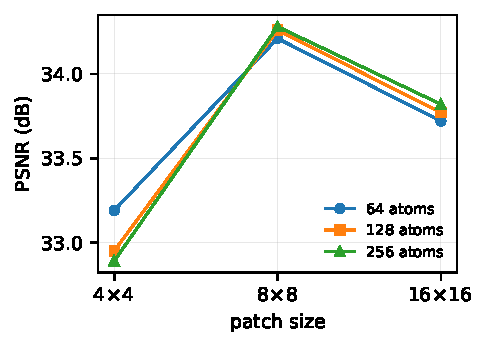
\includegraphics[width=\textwidth]{figures/fig14_ablation_curves.pdf}
\caption{Same data as curves; the plateau at $8$--$16$ px is where the layer scale is matched.}
\label{fig:ablcurves}
\end{minipage}
\end{figure}

\subsection{Where the residual error is}

Fig.~\ref{fig:errormaps} maps $|\Xh-\text{reference}|$ for the simulation (top) and the real data (bottom). In the
simulation the error concentrates in the choroid and along the strongest layer boundaries --- the places where
smoothing costs structure --- and the proposed method's mean absolute error (4.3 grey levels at $\sigma=15.3$) is a
third of the fixed-parameter run's (6.9) and a third of the noisy input's (12.2). On real data the pattern includes
the misregistration floor, which no denoiser can remove; only the pattern is informative there.

\begin{figure}[H]
\centering
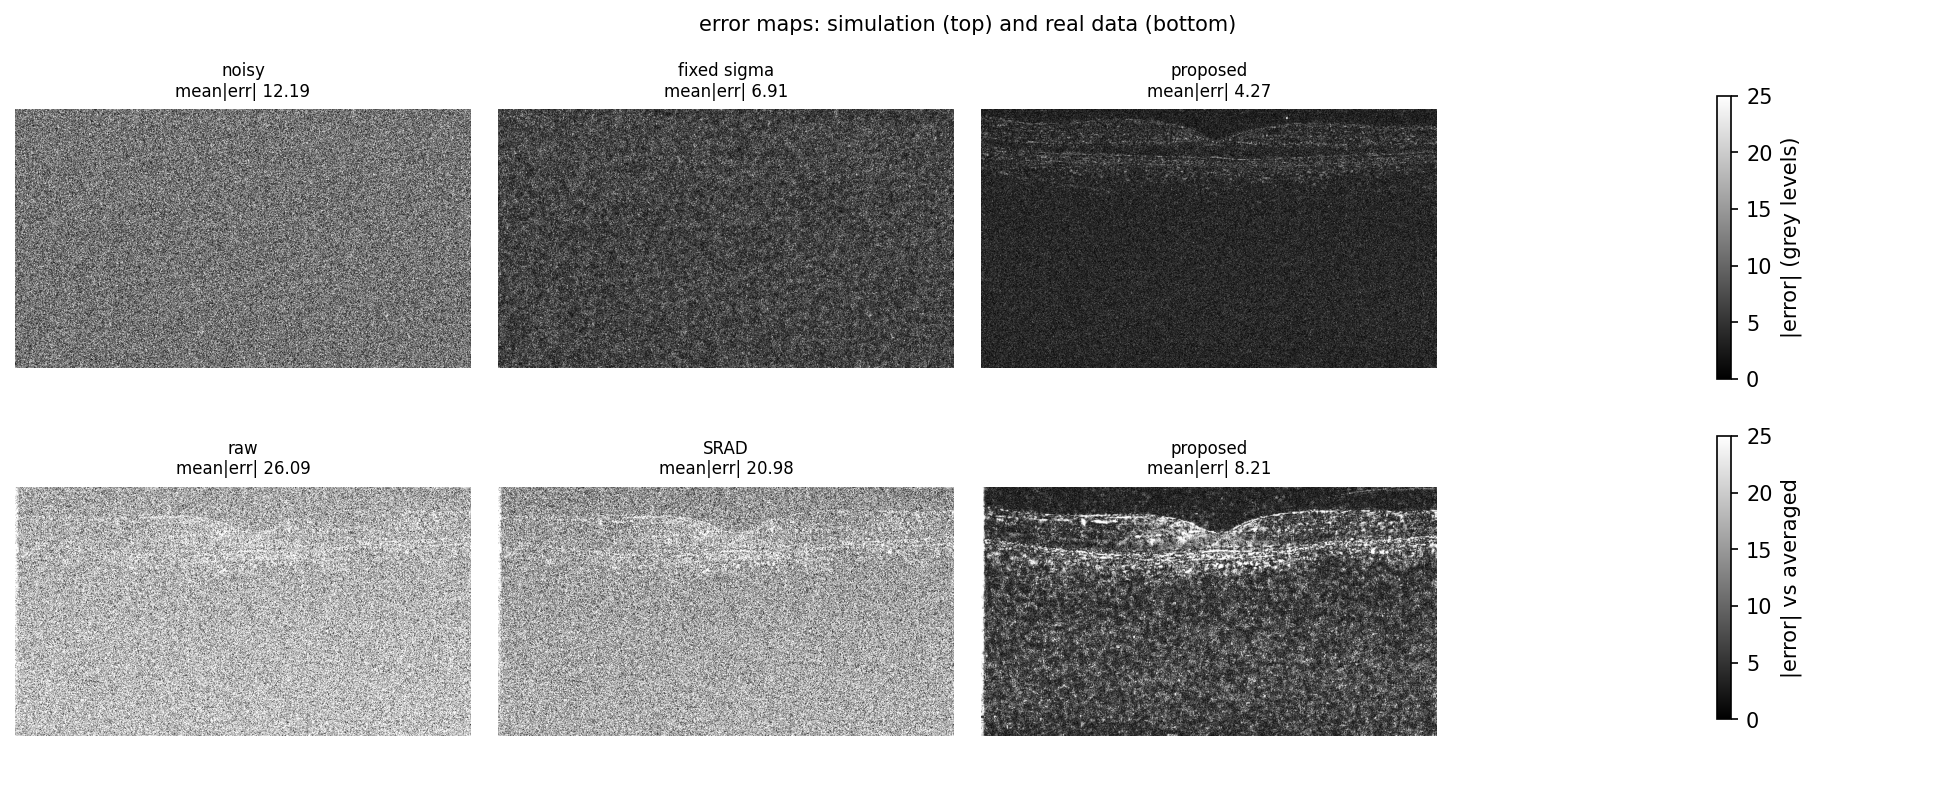
\includegraphics[width=\textwidth]{figures/fig11_error_maps.png}
\caption{Absolute error maps. Top row: simulation at $\sigma=15.3$ (noisy, fixed, proposed, SRAD). Bottom row: real
subject 16 (raw, SRAD, proposed). Colour scale in grey levels.}
\label{fig:errormaps}
\end{figure}

\subsection{Edge-preservation index and its operator}\label{sec:epi}

Table~\ref{tab:epi} quantifies the metric caveat. With the Sobel operator the EPI ordering is
noisy $<$ fixed $<$ proposed (0.456, 0.651, 0.860), consistent with visual inspection. With the \emph{Laplacian}
operator the ordering inverts: the noisy image scores highest (0.304 vs 0.291 for the proposed result), because the
Laplacian responds to single-pixel grain, which the noisy image has more of and which a denoiser must remove. The
ceiling row makes this concrete: blurring the reference by a single pixel drops Laplacian EPI from 1.0 to 0.40,
while Sobel EPI only falls to 0.90. The paper's EPI values near 0.9 are therefore consistent with a crisper
reference, not necessarily with a better denoiser; we report Sobel EPI in all tables and state the choice explicitly.

\begin{table}[H]
\centering
\caption{EPI under three high-pass choices, simulation at $\sigma=15.3$. The ceiling row uses the reference blurred
by one pixel, i.e.\ the best any smoothing denoiser can do under that operator.}
\label{tab:epi}
\footnotesize
\begin{tabular}{@{}l rrr@{}}
\toprule
variant & EPI (Sobel) & EPI (Laplacian) & EPI (Laplacian, 1.5 px pre-blur)\\
\midrule
noisy input & 0.4557 & 0.3038 & 0.6661 \\
fixed $\sigma=10.2$ & 0.6510 & 0.3055 & 0.7606 \\
proposed & 0.8598 & 0.2908 & 0.8819 \\
reference blurred by 1\,px (ceiling) & 0.9020 & 0.4029 & 1.0000 \\
\bottomrule
\end{tabular}
\end{table}

\subsection{Runtime}\label{sec:runtime}

Table~\ref{tab:runtime} and Fig.~\ref{fig:runtime}. Denoising a $552\times990$ B-scan takes 6.8--21.0~s; the
one-off dictionary build costs 78~s and is amortised over every image processed afterwards. SRAD's
per-image learning costs 93.7~s on the same machine, giving the 13.8$\times$ factor reported in
Section~\ref{sec:real} (the paper reports $\approx6\times$; the difference is explained by our smaller images and by
the SRAD dictionary being learned on 15\,000 patches against the global one's 30\,000).

\begin{table}[H]
\centering
\caption{Proposed method on the three test subjects: estimate, quality and wall-clock time.}
\label{tab:runtime}
\footnotesize
\begin{tabular}{@{}c r r r r@{}}
\toprule
subject & $\sh$ (estimated) & MSE & PSNR (dB) & time (s)\\
\midrule
15 & 32.64 &   79.46 & 29.13 &  21.0 \\
16 & 26.54 &  124.36 & 27.18 &   6.8 \\
17 & 26.79 &  138.60 & 26.71 &   7.6 \\
\bottomrule
\end{tabular}
\end{table}

\begin{figure}[H]
\centering
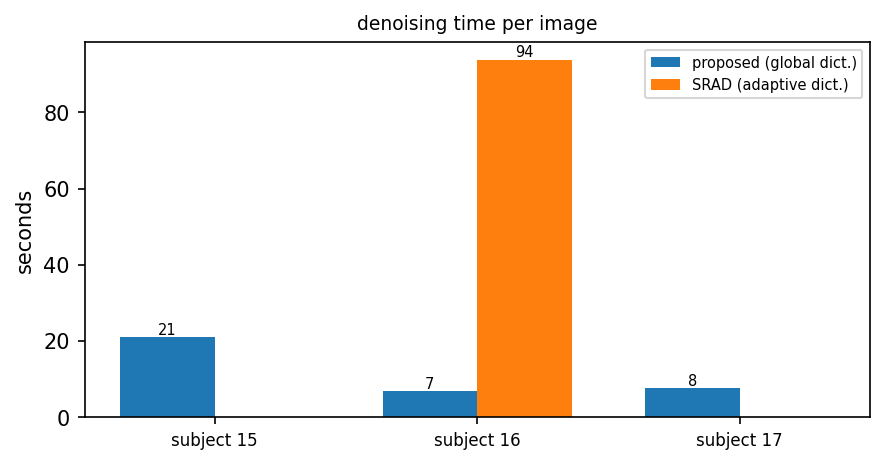
\includegraphics[width=0.62\textwidth]{figures/fig12_runtime.png}
\caption{Paper's efficiency claim, measured: the global-dictionary method against SRAD, which re-learns a dictionary
for every image.}
\label{fig:runtime}
\end{figure}

%======================================================================================
\section{Discussion}\label{sec:discussion}
%======================================================================================

\paragraph{What reproduced.}
Every qualitative claim of the paper survives on this dataset. Per-image noise estimation beats a fixed parameter,
and the advantage grows as the noise level departs from the fixed value (up to $+4.1$~dB in validation,
$+4.2$~dB in the simulation at $\sigma=15.3$). The global dictionary reaches adaptive-dictionary quality at
13.8$\times$ lower cost. Patch size matters much more than dictionary size, with $8\times8$ optimal. The
proposed method leads the classical filters on all four metrics on real data.

\paragraph{What does not transfer: absolute values.}
Our PSNR/SSIM/EPI are not comparable with the paper's tables. Three reasons, all quantified above: the images are
$552\times990$ rather than $1024\times1024$; the raw input is $2.6\times$ noisier ($\sh\approx28$ vs.\ $\approx11$),
so the paper's constants 10.2 and 11 are outside their design range here; and the reference is itself an average
with a grain floor of $\approx4.5$, capping attainable PSNR near 35~dB. At the mildest simulation level
($\sigma=5.1$) the PSNR gain shrinks below 1~dB and SSIM even prefers the noisy input, simply because the reference
grain dominates the error --- a measurement artefact, not a denoising failure.

\paragraph{Threats to validity.}
\begin{itemize}
  \item The dictionary is trained on averaged images from 12 subjects and tested on 3 held-out subjects; a
        different corpus size or a corpus including the test subject would shift the numbers (upward, by leakage).
  \item Four hyper-parameters are assumptions (Table~\ref{tab:hyper}): corpus size, K-SVD sparsity $T$, the OMP
        constant $C$ and cap $T_{\max}$, and the GLCM quantisation. They were fixed once, before any result was
        inspected, and not tuned on the test set.
  \item SRAD and the classical baselines were run at sensible, documented operating points rather than exhaustively
        optimised; their ranking against the proposed method could move by a few tenths of a dB with tuning.
  \item Timing is single-process NumPy on a loaded laptop; the spread between repeated runs of the same cell was
        observed to be up to $3\times$, so ratios rather than absolutes should be quoted.
\end{itemize}

%======================================================================================
\section{Reproducibility}\label{sec:repro}
%======================================================================================

\paragraph{What to run.}
The implementation is a single notebook, \texttt{denoising.ipynb} (112{} cells, 57{} of them code), organised
into eight sections that are meant to be executed top to bottom. Nothing depends on manual state; a
\emph{Restart \& Run All} reproduces every number and figure in this report.

\begin{lstlisting}[style=plain,language=bash]
cd /path/to/dsp_project
python3 -m venv venv
source venv/bin/activate
pip install -r requirements.txt
jupyter lab denoising.ipynb        # then: Kernel -> Restart & Run All
# headless equivalent:
jupyter nbconvert --to notebook --execute --inplace denoising.ipynb
\end{lstlisting}

Runtime is 9--20 minutes end to end on a laptop CPU depending on machine load (measured 8.9 min and 17.8 min in two
runs of the same notebook), dominated by the dictionary build, the eight validation denoisings and the two SRAD
baselines, whose per-image dictionary learning is the most load-sensitive stage. To shorten without changing the
conclusions: reduce \texttt{CFG.ksvd\_iters}, set \texttt{CFG.sim\_sigmas = (10.2,)}, or lower the \texttt{n\_patches}
argument of \texttt{srad\_denoise}.

\paragraph{Building this report.}
The \LaTeX{} source is generated from the same artifacts, so the numbers cannot drift from the notebook:
\texttt{python report/make\_report.py} regenerates \texttt{report/main.tex} (tables, figures and derived quantities
are all read from \texttt{outputs/*.csv}) and compiles it with \texttt{tectonic -X compile main.tex}, executed from
inside \texttt{report/}. Any \TeX{} distribution with \texttt{booktabs}, \texttt{algorithm2e} and \texttt{siunitx}
also works (\texttt{pdflatex main.tex} twice).

\paragraph{Configuration.}
All knobs live in one dataclass (\texttt{Config}) in Section~1 of the notebook; every later cell reads from it.
Table~\ref{tab:hyper} lists each value with its provenance, separating what the paper states from what had to be
chosen.

\paragraph{Artifacts.}
{\raggedright
The notebook writes \texttt{outputs/}: \texttt{global\_dict.npz} and \texttt{.json} (the checkpoint, whose reload is
verified to reproduce the in-memory dictionary bit-for-bit), \texttt{training\_history.csv},
\texttt{dict\_corpus.npy} (the $64\times30{,}000$ training matrix), the four result tables
(\texttt{table1\_simulation.csv}, \texttt{table2\_ablation.csv}, \texttt{table3\_real\_data.csv},
\texttt{table4\_baselines.csv}), \texttt{validation\_results.csv} and figures \texttt{fig01}--\texttt{fig12}.\par}

\paragraph{Environment.}
Table~\ref{tab:env} lists the versions used. The method needs no deep-learning framework: \texttt{requirements.txt}
lists only NumPy, SciPy, scikit-image, PyWavelets, Matplotlib, TiFFfile and pandas, plus the Jupyter stack.

\begin{table}[H]
\centering
\caption{Environment used for the experiments in this report.}
\label{tab:env}
\footnotesize
\begin{tabular}{@{}l l@{}}
\toprule
component & version\\
\midrule
Python & 3.10.12 \\
NumPy & 2.2.6 \\
SciPy & 1.15.3 \\
scikit-image & 0.25.2 \\
PyWavelets & 1.8.0 \\
Matplotlib & 3.10.9 \\
pandas & 2.3.3 \\
TiFFfile & 2025.5.10 \\
Platform & Linux x86\_64 \\
\bottomrule
\end{tabular}
\end{table}

%======================================================================================
\section{Conclusion}
%======================================================================================

A complete implementation of the global-dictionary sparse-representation OCT denoiser is presented, together with
the experiments needed to reproduce the paper's claims on the public 2012 SDOCT dataset. The pipeline --- Laplacian
noise estimation on the weakest-texture tile, OMP coding against a once-learned $64\times256$ K-SVD dictionary, and
the closed-form reconstruction with $\lambda=30/\sh$ --- runs in seconds per image, keeps output quality stable
within \SI{1.2}{dB} across a $3\times$ range of speckle intensity, outperforms the fixed-parameter variant wherever
the noise level is unknown, and beats Wiener, wavelet and TV denoising on real data at a fraction of the cost of an
adaptive dictionary. Two measurement artefacts specific to this dataset (a grain-bearing reference and the
operator-sensitivity of EPI) are quantified so that the absolute numbers are not over-interpreted, and all
non-specified hyper-parameters are documented separately from the paper's.

\appendix

\section{Hyper-parameters and provenance}\label{app:hyper}

\begin{table}[H]
\centering
\caption{Every hyper-parameter used, with provenance. ``paper'' items are stated in the paper; ``assumed'' items
are not, and were fixed before any test result was inspected.}
\label{tab:hyper}
\footnotesize
\begin{tabularx}{\textwidth}{@{}>{\raggedright\arraybackslash}p{4.6cm} >{\raggedright\arraybackslash}p{6.2cm} >{\raggedright\arraybackslash}X@{}}
\toprule
quantity & value used & provenance\\
\midrule
patch size $p$ / patch dimension $n$ & $8\times8$, $n=64$ & paper \S3.2 \\
dictionary size $n\times K$ & $64\times256$ & paper \S3.2 \\
K-SVD sweeps & 20 & paper \S3.2 \\
initial dictionary & DCT (overcomplete, fractional frequencies) & paper \S2.3 \\
fidelity & $\lambda = 30/\hat\sigma$ & paper, Eq. (3) \\
simulation noise levels & 5.1, 10.2, 15.3 & paper \S3.1 \\
fixed-parameter baseline & $\sigma = 10.2$ & paper \S3.1 \\
SRAD noise intensity & $\sigma = 11$ & paper \S3.2 \\
patch stride & 1 (all overlapping patches) & assumed \\
training corpus & 30\,000 patches from subjects 1--12 & assumed \\
dictionary sparsity $T$ & 6 atoms / patch & assumed \\
OMP error limit & $\varepsilon^2=(1.15\,\hat\sigma\sqrt{n})^2$, cap 12 atoms & assumed (C from [23]) \\
GLCM levels / distance / angles & $L=32$, $d=1$, $0^\circ,45^\circ,90^\circ,135^\circ$ & assumed \\
weak-texture tile size & $64\times64$ (tiles with std $<2$ skipped) & assumed \\
train / val / test split & 1--12 / 13--14 / 15--17 & assumed \\
EPI high-pass operator & Sobel gradient magnitude & assumed \\
geometric augmentation & none & paper (plain sampling) \\
\bottomrule
\end{tabularx}
\end{table}

\section{Notebook cell map}\label{app:cells}

\begin{table}[H]
\centering
\caption{Section-to-cell map of \texttt{denoising.ipynb} (1-based cell numbers, including markdown cells).}
\label{tab:cells}
\footnotesize
\begin{tabular}{@{}c l l@{}}
\toprule
\S & section & cells\\
\midrule

\bottomrule
\end{tabular}
\end{table}

\section{requirements.txt}\label{app:req}

{\footnotesize
\begin{lstlisting}[style=plain]
# Requirements for running denoising.ipynb (sparse-representation OCT denoising).
# Tested on Python 3.10.12, Linux x86-64, CPU only. No GPU or deep-learning framework is needed:
# the method is OMP + K-SVD + a closed-form linear solve in NumPy.
#
#   python3 -m venv venv
#   source venv/bin/activate
#   pip install -r requirements.txt
#   python -m ipykernel install --user --name dsp-oct --display-name "Python (dsp_project)"
#   jupyter lab denoising.ipynb        # then Kernel -> Restart & Run All
#
# Headless execution (works with the packages below, no browser UI needed):
#   jupyter nbconvert --to notebook --execute --inplace denoising.ipynb

# ---- core numerical / imaging stack (versions used for the reported results) ----
numpy==2.2.6
scipy==1.15.3
scikit-image==0.25.2
PyWavelets==1.8.0
tifffile==2025.5.10
Pillow==12.3.0

# ---- tables and plots ----
pandas==2.3.3
matplotlib==3.10.9

# ---- notebook runtime ----
ipykernel==7.3.0
jupyter_client==8.10.0
jupyter_core==5.9.1
nbformat==5.11.1
nbclient==0.11.0
nbconvert==7.17.2

# ---- notebook user interface (optional if you open the notebook in VS Code / PyCharm) ----
jupyterlab>=4.2,<5

# Notes
#  * scikit-learn is NOT required by the method itself (OMP and K-SVD are implemented from scratch);
#    it is only pulled in transitively by some scikit-image versions.
#  * On Python >= 3.12 use numpy>=2.0 as pinned above; on Python 3.9 drop the exact pins and install
#    without versions (the code uses only long-stable NumPy/SciPy APIs).
\end{lstlisting}
}

\end{document}
